% !TeX root=SBUKThesis-main.tex
\clearpage
\thispagestyle{empty}
\chapter{پیشینه تحقیق و مفاهیم پایه}\label{chap2}
\section{مقدمه}
مدل‌های زبانی بزرگ بر اساس داده‌های متنی گسترده آموزش دیده و قابلیت درک و تولید زبان طبیعی را دارند. عملکرد این مدل ها بر پایه پیش‌بینی کلمات بعدی در یک جمله یا به عبارتی تکمیل متون بر اساس ورودی داده‌شده است.  

در سال‌های اخیر، مدل‌های زبانی بزرگ رشد چشمگیری داشته\/اند و به دنبال این رشد، ایده استفاده از این مدل ها در تمامی زمینه‌های پردازش زبان طبیعی مورد توجه قرار گرفته است. قابلیت یادگیری مبتنی بر محتوا
\LTRfootnote{In-context Learning}
، که باعث میشود مدل‌ها به ورودی‌های دریافتی دقت ویژه‌ای کنند، کیفیت متن تولید شده جدید را به متن ورودی وابسته میکند. فلذا مهندسی اعلان یکی از اجزای کلیدی در بهبود عملکرد مدل‌های زبانی  است. با طراحی دقیق اعلان‌ها، می‌توان ورودی‌های مدل را به گونه‌ای تنظیم کرد که پاسخ‌های تولیدی با اهداف و نیازهای خاص همخوانی بیشتری داشته باشند. این فرایند نه تنها به بهبود کیفیت و دقت خروجی‌های مدل کمک می‌کند، بلکه در کنترل و هدایت رفتار آن در مواجهه با وظایف مختلف نقش حیاتی دارد. استفاده از مهندسی اعلان زمینه‌ساز تطبیق بهتر مدل با شرایط متغیر و کاهش ابهامات در تولید جواب است.

مسئله اصلی این تحقیق، چالش‌های موجود در طراحی دستی اعلان‌هاست که به دلیل پیچیدگی و زمان‌بر بودن، نیازمند راهکارهایی خودکار می‌باشد. در این راستا، هدف این تحقیق ارائه روشی مبتنی بر الگوریتم جستجو در فضای اعلان‌ها برای تولید خودکار اعلان‌های بهینه است. این رویکرد می‌تواند باعث بهبود دقت و کارایی مدل‌های زبانی شده و از بروز خطاهای ناشی از طراحی دستی جلوگیری کند.

\section{بررسی مدل‌های زبانی بزرگ}
مدل‌های زبانی بزرگ سیستم‌های پیشرفته‌ای هستند که با بهره‌گیری از تکنیک‌های یادگیری عمیق، توانایی پردازش و تولید زبان طبیعی را به سطحی بالا رسانده‌اند. این مدل‌ها با تحلیل حجم عظیمی از داده‌های متنی، قادر به درک مفاهیم، استخراج اطلاعات و تولید متونی دقیق و معنادار می‌باشند. از کاربردهای آن‌ها می‌توان به ترجمه، خلاصه‌سازی، پاسخگویی به سوالات و حتی تولید محتوا در حوزه‌های مختلف اشاره کرد.

تحولات اخیر در این حوزه، مسیر توسعه و بهبود این مدل‌ها را هموار ساخته است. شناخت تاریخچه و معماری این مدل‌ها نقش مهمی در درک عملکرد و پتانسیل‌های آن‌ها دارد که در ادامه به آن می\/پردازیم.

\subsection{تاریخچه و تکامل مدل‌ها}

تکامل مدل‌های زبانی، مسیر پیچیده‌ای از رویکردهای اولیه‌ی مبتنی بر قواعد نمادین تا استفاده از شبکه‌های عصبی پیشرفته و معماری‌های نوین مانند ترنسفورمر را در بر می‌گیرد. در ادامه به تفصیل به بررسی مراحل مختلف این تکامل پرداخته می‌شود.

\textbf{دوران اولیه: رویکردهای نمادین و قواعد دست‌نویس}

\noindent در دهه‌های ۱۹۵۰ و ۱۹۶۰، اولین تلاش‌ها برای پردازش زبان طبیعی به وسیله‌ی روش‌های نمادین انجام شد. پژوهشگران در آن زمان سعی می‌کردند ساختارهای دستوری و قوانین زبان را به صورت صریح و دستی تعریف کنند. این رویکردها با وجود تلاش‌های ارزشمند، به دلیل محدودیت‌های محاسباتی و عدم وجود داده‌های کافی، نتوانستند به دقت و کارایی مورد انتظار دست یابند.

\textbf{ورود به عصر آماری}

\noindent با گذر زمان و ورود به دهه‌های ۱۹۶۰ و ۱۹۷۰، رویکردهای آماری جایگزین بخش‌هایی از روش‌های نمادین شدند. در این دوران، مدل‌های \lr{n-gram} که بر مبنای احتمال وقوع یک کلمه با توجه به کلمات قبلی محاسبه می‌شدند، به عنوان اولین قدم‌های موفق در مدلسازی زبان مطرح شدند. اگرچه این مدل‌ها ساده بودند، اما توانستند برخی از پیچیدگی‌های اولیه‌ی پردازش زبان را کاهش دهند.

\textbf{ظهور یادگیری ماشین و شبکه‌های عصبی}

\noindent در دهه‌های ۱۹۸۰ و ۱۹۹۰، با پیشرفت‌های چشمگیر در فناوری‌های محاسباتی و افزایش دسترسی به داده‌های متنی، روش‌های یادگیری ماشین وارد عرصه شدند. الگوریتم‌های یادگیری نظارت‌شده و غیرنظارتی به منظور تشخیص الگوهای زبانی به کار گرفته شدند. با این حال، محدودیت‌های موجود همچنان مانع از دستیابی به درک عمیق‌تر و تولید متن‌های طبیعی به سطح امروزی می‌شدند.

\textbf{عصر شبکه‌های عصبی عمیق}

\noindent ورود به قرن ۲۱ و به‌ویژه دهه ۲۰۱۰، با ظهور شبکه‌های عصبی عمیق مانند شبکه‌های عصبی بازگشتی
\LTRfootnote{Recursive Neural Networks (RNNs)}
 و شبکه‌های حافظه بلندمدت
\LTRfootnote{Long short-term memory (LSTM)}
  همراه بود. این مدل‌ها توانستند وابستگی‌های زمانی و روابط بلندمدت موجود در متن را بهتر مدل‌سازی کنند. با این حال، چالش‌هایی همچنان در زمینه بهبود کیفیت و کارایی تولید متن وجود داشت.

\textbf{انقلاب ترنسفورمر و ظهور مدل‌های بزرگ}

\noindent نقطه عطف مهم در تکامل مدل‌های زبانی، معرفی معماری ترنسفورمر 
\cite{attention}
 بود. این معماری با بهره‌گیری از مکانیزم توجه
\LTRfootnote{Attention Mechanism}
  توانست وابستگی‌های بین کلمات را به صورت موازی و با کارایی بالا پردازش کند. ویژگی‌های کلیدی ترنسفورمر شامل پردازش موازی داده‌ها، درک بهتر وابستگی‌های طولانی‌مدت در متن و افزایش سرعت و بهبود کارایی مدل‌های زبانی است.

\textbf{توسعه مدل‌های پیشرفته مانند GPT و BERT}

\noindent با معرفی ترنسفورمر، مدل‌های بزرگی نظیر GPT و BERT توسعه یافتند:
\begin{itemize}
	\item GPT
	\LTRfootnote{Generative Pre-trained Transformer}
	: این مدل ها با افزایش تعداد پارامترها (به عنوان مثال، GPT-3 با ۱۷۵ میلیارد پارامتر) توانسته‌اند وظایفی مانند ترجمه، خلاصه‌سازی و پاسخ به سؤالات را با دقت بسیار بالا انجام دهند.
	\item BERT
	\LTRfootnote{Bidirectional Encoder Representations from Transformers}
	: این مدل با تمرکز بر درک بهتر معنایی کلمات در متن، در وظایف مختلف پردازش زبان عملکرد قابل‌توجهی از خود نشان داده است.
\end{itemize}

\textbf{تکنیک‌های بهبود عملکرد: تنظیم دقیق و یادگیری انتقالی}

\noindent علاوه بر افزایش تعداد پارامترها و مقیاس داده‌های آموزشی، تکنیک‌هایی مانند تنظیم دقیق
\LTRfootnote{Fine-tuning}
 و یادگیری انتقالی
\LTRfootnote{Transfer Learning}
  نقش مهمی در بهبود عملکرد مدل‌های زبانی داشته‌اند. این تکنیک‌ها امکان تطبیق مدل‌های پیش‌آموزش داده شده با وظایف خاص را فراهم می‌آورند که باعث بهبود کیفیت و دقت در کاربردهای متنوع می‌شود.


پیشرفت‌های حاصل از توسعه مدل‌های زبانی بزرگ، مرزهای جدیدی در تعامل انسان و ماشین ایجاد کرده است. سیستم‌های هوشمند مبتنی بر این مدل‌ها قادرند که به صورت طبیعی و انسانی با کاربران تعامل کنند، همچنین در زمینه‌های مختلفی از جمله خدمات مشتری، ترجمه ماشینی، تحلیل متون و تولید محتوا به کار گرفته شوندو وظایف پیچیده زبانی را با دقت و سرعت بالا انجام دهند.


تکامل مدل‌های زبانی از روش‌های نمادین اولیه به سوی استفاده از شبکه‌های عصبی عمیق و معماری‌های پیشرفته مانند ترنسفورمر، نشان‌دهنده یک مسیر پرفراز و نشیب اما پر از نوآوری است. این پیشرفت‌ها بهبود قابل‌توجهی در درک و تولید زبان انسانی ایجاد کرده و نقش مهمی در توسعه فناوری‌های هوش مصنوعی و تعامل انسان-ماشین داشته‌اند.


\subsection{معماری‌ها و کاربردهای اصلی}
در ادامه، به تفصیل به بررسی معماری‌های کلیدی این مدل‌ها می‌پردازیم.
\begin{enumerate}
	\item \textbf{معماری ترنسفورمر}
	\LTRfootnote{Transformer}\textbf{:}
	معماری ترنسفورمر پایه و اساس بسیاری از مدل‌های زبانی بزرگ است. این معماری با استفاده از مکانیزم توجه
	\LTRfootnote{Attention Mechanism}
	، امکان پردازش موازی داده‌ها و درک وابستگی‌های طولانی‌مدت در متن را فراهم می‌کند. برخلاف مدل‌های پیشین که بر پایه شبکه‌های عصبی بازگشتی
	\LTRfootnote{Recursive Neural Networks}
	 بودند، ترنسفورمرها با حذف وابستگی‌های ترتیبی، کارایی و سرعت پردازش را بهبود بخشیدند. دیاگرام این معماری در شکل \ref{fig_transformer} نمایش داده شده است.
	 \begin{figure}[!t]
	 	\centering
	 	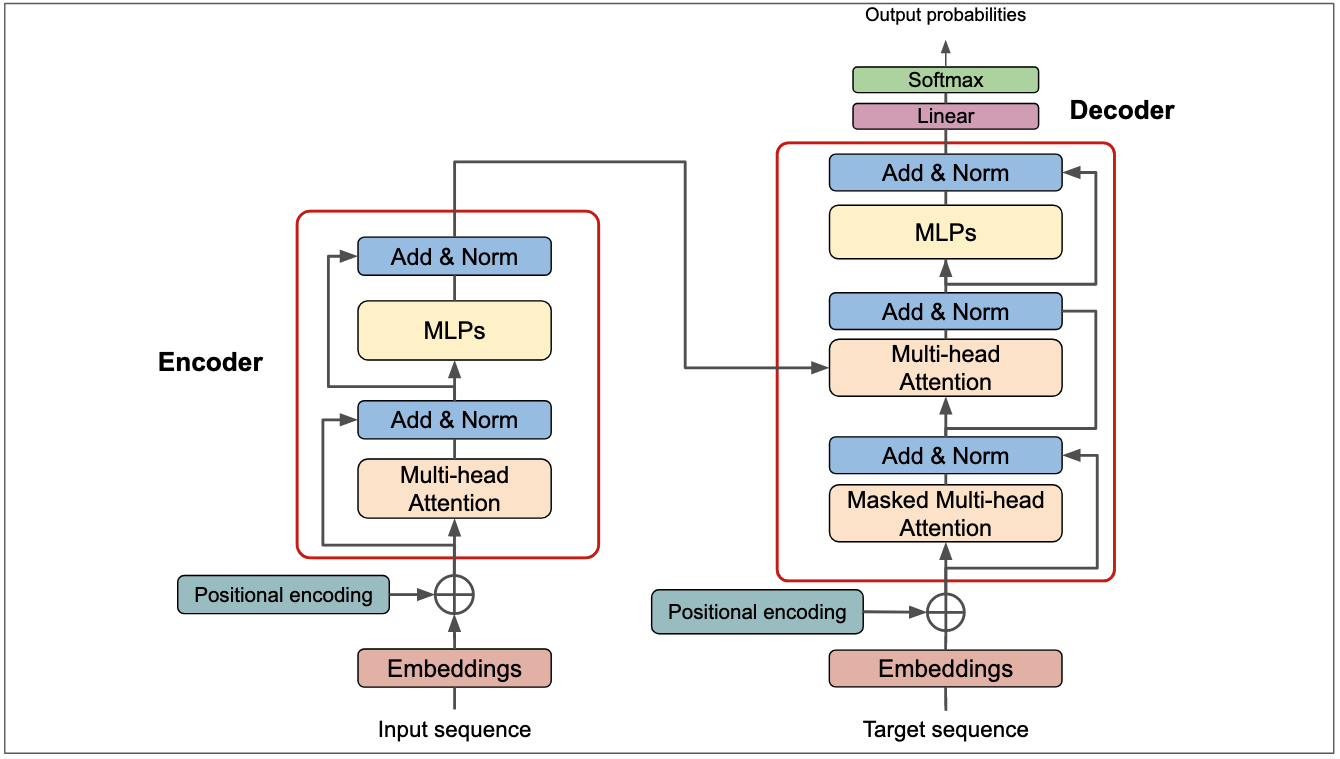
\includegraphics[width=140mm]{images/transformer}
	 	\caption{دیاگرام معماری ترنسفورمر }
	 	\label{fig_transformer}
	 \end{figure}
	 
	\item \textbf{مکانیزم توجه:}
	مکانیزم توجه به مدل‌ها اجازه می‌دهد تا به بخش‌های مختلف ورودی با وزن‌های متفاوت نگاه کنند و وابستگی‌های معنایی را بهتر درک نمایند. این مکانیزم به‌ویژه در ترجمه ماشینی و خلاصه‌سازی متون کاربرد دارد.
	
	\item \textbf{معماری‌های خودبازگشتی}
	\LTRfootnote{Autoregressive}
	\textbf{ و خودرمزگذار}
	 \LTRfootnote{Autoencoder}\textbf{:}
	\begin{itemize}
		\item 
	مدل‌های خودبازگشتی مانند سری GPT متن را به‌صورت ترتیبی تولید می‌کنند و هر کلمه را بر اساس کلمات قبلی پیش‌بینی می‌نمایند.
		\item 
	مدل‌های خودرمزگذار مانند BERT با استفاده از ماسک‌کردن کلمات در ورودی، سعی در درک زمینه و پیش‌بینی کلمات ماسک‌شده دارند.
	\end{itemize}
\end{enumerate}

\subsection{مدل بزرگ زبانی Mistral}


مدل بزرگ زبانی Mistral \cite{mistral} از جمله دستاوردهای جدید در حوزه پردازش زبان طبیعی به شمار می‌آید که با بهره‌گیری از معماری ترنسفورمر، عملکرد بالایی در وظایف متنوع زبانی نشان داده است. در ادامه به بررسی جامع این مدل می‌پردازیم.

مدل Mistral بر پایه معماری ترنسفورمر طراحی شده است. همانطور که گفته شد، این معماری با استفاده از مکانیزم توجه قادر است وابستگی‌های طولانی‌مدت در متون را به‌صورت موازی پردازش کند. از ویژگی‌های برجسته این مدل می‌توان به استفاده از تعداد پارامترهای بالا
\footnote{در این پژوهش از مدل‌های 7 میلیارد پارامتری استفاده شده است}
 اشاره کرد که موجب بهبود دقت و کیفیت تولید متن می‌شود.

برای رسیدن به عملکرد مطلوب، مدل Mistral با استفاده از مجموعه‌های داده گسترده و متنوع آموزش داده شده است. علاوه بر این، بهره‌گیری از تکنیک‌های تنظیم دقیق
\LTRfootnote{Fine-tuning}
 و بهینه‌سازی پیشرفته، موجب شده تا مدل بتواند در وظایف خاص، همچون ترجمه، خلاصه‌سازی و پاسخ به پرسش، عملکرد بهتری از خود نشان دهد.


مدل Mistral در حوزه‌های مختلف پردازش زبان طبیعی کاربرد دارد. از وظایف مهم آن می\/توان به توانایی تولید متونی با کیفیت بالا و طبیعی، ارائه ترجمه‌های دقیق و روان بین زبان‌ها، استخراج اطلاعات کلیدی و ارائه خلاصه‌های مفید از متون طولانی و همچنین درک دقیق سوالات و ارائه پاسخ‌های مرتبط و دقیق اشاره کرد.


با وجود این توانایی ها، مدل Mistral دارای نوآوری‌ها و مزایای متعددی نیز است که آن را از سایر مدل‌های زبانی متمایز می‌کند. این نوآوری ها شامل بهره‌گیری از معماری ترنسفورمر جهت پردازش موازی و بهبود سرعت محاسبات است، همچنین استفاده از تعداد پارامترهای بالا به افزایش دقت و کیفیت خروجی‌ها منجر می‌شود و قابلیت تنظیم دقیق برای تطبیق با وظایف خاص و کاربردهای صنعتی و پژوهشی را فراهم می آورد و به دنبال آن، بهبود چشمگیری در درک وابستگی‌های زبانی و تولید متون طبیعی حاصل می\/شود.


با وجود دستاوردهای قابل توجه، مدل Mistral همچنان با چالش‌هایی همچون مصرف بالای منابع محاسباتی و نیاز به داده‌های آموزشی گسترده مواجه است. پژوهش‌های آتی در زمینه بهبود کارایی، کاهش هزینه‌های محاسباتی و افزایش دقت در کاربردهای خاص، افق‌های روشن‌تری را برای این مدل ترسیم می‌کند.



\section{مهندسی اعلان}
مهندسی اعلان 
\LTRfootnote{Prompt Engineering}
 به فرآیند طراحی و بهینه‌سازی ورودی‌های متنی اطلاق می‌شود که به مدل‌های زبانی بزرگ ارائه می‌گردد تا خروجی‌های مطلوب و دقیقی تولید کنند. این ورودی‌ها می‌توانند شامل دستورات، سؤالات یا داده‌های زمینه‌ای باشند که به مدل کمک می‌کنند تا پاسخ‌های خود را در چارچوب معنایی و ساختاری مشخصی ارائه دهد.
می\/دانیم که مهندسی اعلان تأثیر مستقیمی بر کارایی و دقت مدل‌های زبانی بزرگ دارد از این رو با تدوین اعلان‌های دقیق و متناسب با وظیفه موردنظر، می‌توان رفتار مدل را به‌گونه‌ای هدایت کرد که خروجی‌های مرتبط‌تر و با کیفیت‌تری تولید کند. این امر به‌ویژه در شرایطی که داده‌های آموزشی محدود یا ناموجود هستند، اهمیت بیشتری پیدا می‌کند.
از مزایای مهندسی اعلان میتوان به موارد زیر اشاره کرد :
\begin{itemize}
	\item 
	با استفاده از اعلان‌های دقیق و مناسب می‌توان نتایج مدل را به سمت پاسخ‌های موردنظر هدایت کرد و کنترل بیشتری بر خروجی مدل داشت.
	\item 
	مهندسی اعلان می‌تواند به کاهش سوگیری‌های موجود در مدل‌های زبانی کمک کند و نتایج منصفانه‌تری ارائه دهد.
	\item 
	با تدوین اعلان‌های مؤثر، می‌توان زمان و منابع موردنیاز برای رسیدن به نتایج مطلوب را کاهش داد و کارایی را افزایش داد.
\end{itemize}

در نتیجه، مهندسی اعلان به‌عنوان ابزاری قدرتمند برای بهبود عملکرد مدل‌های زبانی بزرگ محسوب می‌شود و نقش کلیدی در توسعه و بهره‌برداری مؤثر از این مدل‌ها ایفا می‌کند.

\section{روش‌های دستی در مهندسی اعلان}
مهندسی اعلان دستی به فرآیند طراحی و بهینه‌سازی دستی ورودی‌ها (اعلان‌ها) برای هدایت بهتر مدل‌های زبانی بزرگ در تولید پاسخ‌های مطلوب گفته می‌شود. برخلاف روش‌های خودکار که از الگوریتم‌های یادگیری ماشین برای بهینه‌سازی اعلان‌ها استفاده می‌کنند، روش‌های دستی بر دانش زبانی، شهود انسانی و آزمایش‌های مکرر متکی هستند. این تکنیک‌ها در کاربردهای واقعی که نیاز به کنترل دقیق بر خروجی مدل دارند، مانند پاسخ‌گویی به سوالات، خلاصه‌سازی متون و انجام وظایف استدلالی، به‌کار گرفته می‌شوند.  

مهندسی اعلان دستی برای افزایش اثربخشی مدل‌های زبانی ضروری است، به‌ویژه در مواردی که تنظیم و آموزش مجدد مدل امکان‌پذیر نیست. از آنجایی که مدل‌های زبانی پاسخ‌های خود را بر اساس ورودی‌ها تولید می‌کنند، حتی تغییرات جزئی در ساختار یا نحوه بیان اعلان‌ها می‌تواند تأثیر قابل‌توجهی بر عملکرد آن‌ها داشته باشد. اعلان‌های طراحی‌شده به‌صورت بهینه می‌توانند دقت مدل را افزایش داده، توانایی استدلال آن را بهبود بخشند و میزان سوگیری در پاسخ‌ها را کاهش دهند، در نتیجه پاسخ‌های دقیق‌تر و متناسب‌تری ارائه کنند.

از ویژگی‌های کلیدی مهندسی اعلان دستی میتوان به موارد زیر اشاره کرد :
\begin{enumerate}
	\item طراحی مبتنی بر دانش انسانی 
	\begin{itemize}
		\item برخلاف روش‌های خودکار که از الگوریتم‌های بهینه‌سازی استفاده می‌کنند، مهندسی اعلان دستی بر شهود انسانی و دانش زبانی تکیه دارد.
		\item درک صحیح از زبان و زمینه موردنظر نقش مهمی در طراحی اعلان‌هایی دارد که مدل را به تولید خروجی‌های مطلوب هدایت می‌کنند. 
	\end{itemize}
	
	\item بهینه‌سازی تدریجی و تکرارشونده
	\begin{itemize}
		\item طراحی اعلان‌های مؤثر نیازمند آزمایش‌های مداوم و اصلاحات متوالی است. 
		\item تنظیمات و تغییرات مداوم در نحوه بیان اعلان به شناسایی بهترین ساختار و سبک ورودی کمک می‌کند. 
	\end{itemize}
	
	\item انعطاف‌پذیری در کاربردهای مختلف
	\begin{itemize}
		\item مهندسی اعلان دستی امکان شخصی‌سازی ورودی‌ها را برای وظایف متنوعی مانند تولید محتوا، برنامه‌نویسی و استدلال منطقی فراهم می‌کند.  
		\item استراتژی‌های خاصی را می‌توان برای هر کاربرد به‌کار گرفت، مانند ارائه دستورالعمل‌های گام‌به‌گام، اضافه کردن نشانه‌های متنی یا استفاده از نمونه‌های مشابه.
	\end{itemize}
	
	\item کنترل و تفسیرپذیری بهتر
	\begin{itemize}
		\item از آنجا که اعلان‌های دستی توسط انسان طراحی می‌شوند، کنترل بیشتری بر رفتار مدل فراهم می‌کنند.  
		\item این روش امکان درک بهتر نحوه پاسخ‌گویی مدل به ورودی‌های مختلف را فراهم کرده و به عیب‌یابی و بهبود عملکرد کمک می‌کند.
	\end{itemize}
\end{enumerate}

با وجود مزایای فراوان، این روش با چالش‌هایی همراه است:  
\begin{itemize}
	\item فرآیند زمان‌بر: طراحی و بهینه‌سازی دستی اعلان‌ها نیاز به صرف زمان زیادی دارد.  
	\item مقیاس‌پذیری پایین: برخلاف روش‌های خودکار، اعلان‌های دستی به‌راحتی برای مدل‌ها یا وظایف دیگر تعمیم نمی‌یابند.  
	\item ماهیت مبتنی بر آزمون و خطا: یافتن اعلان بهینه اغلب نیازمند آزمایش‌های متعدد است که همیشه نتیجه‌ای ثابت و پایدار را تضمین نمی‌کند.  
\end{itemize}

در نهایت مهندسی اعلان دستی به‌عنوان رویکردی بنیادین برای بهینه‌سازی تعاملات با مدل‌های زبانی شناخته می‌شود. در بخش‌های بعدی، روش‌های مختلف مهندسی اعلان دستی را بررسی خواهیم کرد و تأثیر هر یک را بر توانایی‌های استدلالی و کیفیت پاسخ‌دهی مدل می‌سنجیم.
%بررسی کاربرد و مزایا و معایب این روش‌ها
\subsection{یادگیری درون متنی}

یادگیری درون‌متنی
\LTRfootnote{In-Context Learning}
 از قابلیت‌های برجسته مدل‌های زبانی بزرگ است که به آن‌ها اجازه می‌دهد بدون نیاز به بازآموزی
 \LTRfootnote{Training}
  یا تنظیم مجدد وزن‌ها، تنها با دریافت چند نمونه در ورودی، وظایف جدید را تشخیص دهند و به درستی انجام دهند. این روش به مدل کمک می‌کند با تحلیل مثال‌های ارائه‌شده در ورودی، پاسخ‌هایی متناسب با همان زمینه تولید کند.
از مزایای مهم این روش، افزایش انعطاف‌پذیری در مواجهه با وظایف و موضوعات جدید است که باعث می\/شود مدل‌های زبانی به سرعت خود را با زمینه‌های مختلف تطبیق دهند. با حذف نیاز به بازآموزی برای هر وظیفه جدید، این روش می‌تواند بهینه‌سازی قابل توجهی در مصرف منابع و زمان ایجاد کند.
از سوی دیگر، این قابلیت نقش مهمی در بهبود کیفیت تعاملات میان انسان و ماشین ایفا می‌کند. مدل‌ها با درک بهتر زمینه و مثال‌های ارائه‌شده، پاسخ‌هایی طبیعی‌تر و دقیق‌تر تولید می‌کنند که باعث افزایش رضایت کاربران می‌شود.

با وجود مزایای فوق، یادگیری درون‌متنی با چالش‌هایی نیز همراه است. عملکرد مدل‌ها به شدت به کیفیت و تنوع داده‌ها و مثال‌های ورودی وابسته است. مثال‌های ناقص یا ناسازگار می‌توانند منجر به تولید پاسخ‌های نادرست شوند. همچنین، در برخی موقعیت‌های پیچیده یا مبهم، مدل ممکن است در درک دقیق زمینه دچار مشکل شود. 


از روش های یادگیری درون متنی میتوان به یادگیری بدون نمونه و یادگیری با نمونه های کم اشاره کرد. در یادگیری بدون نمونه 
\cite{ZSL}
\LTRfootnote{Zero-Shot Learning (ZSL)}
  مدل‌ها وظیفه دارند اشیاء یا مفاهیمی را که در طول آموزش با آن‌ها روبرو نشده‌اند شناسایی و دسته‌بندی کنند. برخلاف یادگیری نظارت‌شده سنتی که نیاز به مثال‌های برچسب‌خورده برای هر کلاس دارد، یادگیری بدون نمونه به مدل‌ها این امکان را می‌دهد که پیش‌بینی‌هایی در مورد دسته‌های دیده نشده در زمان آموزش با استفاده از اطلاعات کمکی انجام دهند.  
برای شناسایی کلاس‌های دیده نشده در زمان آموزش، مدل‌های یادگیری بدون نمونه روابطی بین کلاس‌های مشاهده‌شده (دیده‌شده) و کلاس‌های مشاهده‌نشده (دیده‌ نشده) برقرار می‌کنند. این ارتباط معمولاً از طریق ویژگی‌های مشترک یا اطلاعات معنایی که این دو را به هم پیوند می‌دهند، تسهیل می‌شود.  
از طرفی وجود اطلاعات کمکی برای یادگیری بدون نمونه حیاتی است و  داده‌های توصیفی در مورد کلاس‌های دیده‌شده و دیده نشده ارائه می‌دهد. این اطلاعات می‌تواند شامل ویژگی‌هایی مانند توضیحات متنی، جاسازی‌های معنایی یا سایر داده‌های مرتبط باشد که به مدل کمک می‌کند تا کلاس‌ها را درک کرده و از هم تمایز دهد. 

چگونگی عملکرد یادگیری بدون نمونه بدین صورت است که در غیاب مثال‌های برچسب‌خورده برای کلاس‌های دیده نشده، برای پر کردن شکاف به اطلاعات کمکی اتکا می\/کنند. به عنوان مثال، در طبقه‌بندی تصاویر، مدلی که بر اساس گونه‌های خاص حیوانات آموزش دیده باشد، می‌تواند از توضیحات متنی گونه‌های دیده نشده برای شناسایی صحیح آن‌ها استفاده کند. با درک اینکه یک گورخر مشابه یک اسب است اما با خطوط راه‌راه، مدل می‌تواند گورخرها را بدون دیدن آن‌ها در طول آموزش شناسایی کند (تصویر \ref{fig_zil}).

\begin{figure}[!t]
	\centering
	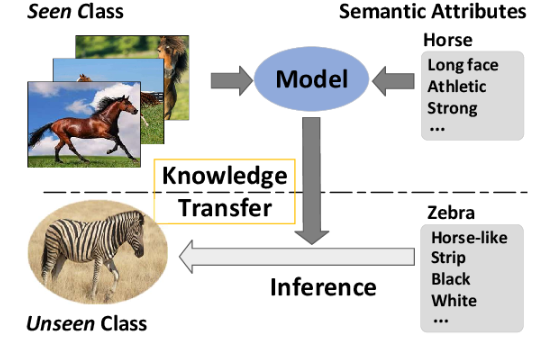
\includegraphics[width=100mm]{images/ZeroShot}
	\caption{مثالی از یادگیری بدون نمونه در یادگیری درون متنی}
	\label{fig_zil}
\end{figure}

یادگیری بدون نمونه در حوزه‌های مختلفی کاربرد داشته است، از جمله:
\begin{itemize}
	\item 
	طبقه‌بندی تصویر: شناسایی اشیاء یا گونه‌هایی که در داده‌های آموزشی وجود ندارند.
	\item 
	بخش‌بندی معنایی: بخش‌بندی اشیاء دیده نشده در تصاویر بر اساس ویژگی‌های یادگرفته‌شده.
	\item 
	پردازش زبان طبیعی: انجام کارهایی مانند طبقه‌بندی متن یا شناسایی موجودیت‌ها بدون مثال‌های صریح.
	\item 
	زیست‌شناسی محاسباتی: پیش‌بینی عملکرد ژن‌ها یا پروتئین‌هایی که فاقد نشانه‌های آزمایشی هستند.  
\end{itemize}

از چالش‌های مهم یادگیری بدون نمونه می\/توان به احتمال اشتباه کردن مدل در دسته‌بندی کلاس‌های دیده نشده اشاره کرد، به ویژه زمانی که این کلاس‌ها ویژگی‌هایی مشابه با کلاس‌های دیده‌شده دارند. تحقیقات جاری به دنبال افزایش کارایی و دقت مدل‌های یادگیری بدون نمونه است و روش‌هایی مانند تولید داده‌های مصنوعی برای کلاس‌های دیده نشده و بهبود کیفیت اطلاعات کمکی را بررسی می‌کنند.

در طرف دیگر ماجرا، برای یادگیری با نمونه های کم \cite{FSL} مدل‌ها طوری طراحی می‌شوند که بتوانند بر اساس تعداد بسیار محدودی از نمونه‌های آموزشی، یادگیری کرده و پیش‌بینی‌های دقیقی انجام دهند. این رویکرد به‌ویژه در موقعیت‌هایی مفید است که جمع‌آوری مجموعه‌داده‌های بزرگ عملی یا مقرون‌به‌صرفه نیست.

در یادگیری با نمونه های کم، مدل‌ها در مرحله استنتاج تنها تعداد کمی نمونه برچسب‌خورده (که اغلب به آن مجموعه پشتیبان
\LTRfootnote{support set}
 گفته می‌شود) برای هر کلاس جدید دریافت می‌کنند. این تعداد محدود از نمونه‌ها به مدل امکان می‌دهد تا به سرعت خود را تطبیق داده و برای کلاس‌های نادیده‌شده پیش‌بینی انجام دهد.

یک تنظیم رایج در یادگیری با نمونه های کم شامل الگوی N-way K-shot است که در آن 'N' نشان‌دهنده تعداد کلاس‌های جدید و 'K' نشان‌دهنده تعداد نمونه‌های برچسب‌خورده موجود برای هر کلاس است. برای مثال، در یک سناریوی 5-way 1-shot، پنج کلاس جدید وجود دارد که هر کدام تنها یک نمونه برچسب‌خورده دارند.

مدل‌های یادگیری با نمونه های کم معمولاً از تکنیک‌های فرا-یادگیری 
\LTRfootnote{meta Learning}
 استفاده می‌کنند که به آن "یادگیری برای یادگیری
 \LTRfootnote{Learning to Learn}
 " نیز گفته می‌شود. در این چارچوب، مدل در طیف وسیعی از وظایف آموزش می‌بیند تا یک استراتژی برای تطبیق سریع با وظایف جدید با حداقل داده‌ها را یاد بگیرد. در زمان استنتاج، مدل با استفاده از همان تعداد اندک نمونه‌ها، پارامترهای خود را به‌طور مؤثری تنظیم می‌کند و می‌تواند دسته‌بندی‌های جدید را شناسایی و طبقه‌بندی کند.

از کاربردهای یادگیری با نمونه‌های کم می\/توان به موارد زیر اشاره کرد:
\begin{itemize}
	\item 
	یادگیری با نمونه‌های کم به مدل‌ها امکان می‌دهد تصاویر را با استفاده از تنها چند نمونه برچسب‌خورده در دسته‌های جدید طبقه‌بندی کنند که این موضوع به‌ویژه در حوزه‌هایی مانند تصویربرداری پزشکی که برچسب‌گذاری داده‌ها بسیار زمان‌بر است، اهمیت دارد.
	\item 
	در حوزه پردازش زبان طبیعی، یادگیری با نمونه‌های کم می‌تواند در وظایفی مانند طبقه‌بندی متن و تحلیل احساسات به کار رود و به مدل‌ها کمک کند تا با حداقل داده متنی، موضوعات جدید را پردازش و درک کنند.
	\item 
	ربات‌ها می‌توانند با استفاده از یادگیری با نمونه‌های کم وظایف جدید در زمینه دست‌کاری اشیاء یا تطبیق با محیط‌های تازه را یاد بگیرند، که این موضوع نیاز به آموزش مجدد گسترده را کاهش داده و امکان استقرار سریع در محیط‌های پویا را فراهم می‌آورد.
\end{itemize}

یکی از چالش‌های اصلی در یادگیری با نمونه‌های کم این است که اطمینان حاصل شود مدل‌ها خود را با داده‌های محدودبه‌خوبی تعمیم می‌دهند و دچار بیش‌برازش
\LTRfootnote{overfitting}
 نمی‌شوند. پژوهشگران در حال بررسی روش‌های مختلفی از جمله افزایش داده 
 \LTRfootnote{data augmentation}
 ، یادگیری انتقالی
 \LTRfootnote{transfer learning}
  و الگوریتم‌های پیشرفته فرا-یادگیری
  \LTRfootnote{meta Learning}
   برای بهبود عملکرد مدل‌های یادگیری با نمونه‌های کم هستند.

برای فهم شفاف تر روش یادگیری درون متنی میتوان از یک چهارچوب ریاضیاتی
\cite{beysian}
 کمک گرفت. در این چارچوب ریاضیاتی می\/توان یادگیری درون‌متنی را به‌عنوان یک استنتاج بیزی ضمنی
\LTRfootnote{implicit Bayesian inference}
 تفسیر کرد. در چارچوب آن‌ها، در طی پیش‌آموزش
 \LTRfootnote{pre-training}
 ، مدل‌های زبانی بزرگ با استنتاج مفاهیم پنهان در اعلان، که روابط معنایی و نحوی مختلفی را در متن در بر می‌گیرد، یاد می‌گیرند که توکن‌های بعدی را پیش‌بینی کنند. در زمان استنتاج
 \LTRfootnote{inference time}
 ، زمانی که مدلی با یک اعلان شامل مثال‌های ورودی-خروجی مواجه می‌شود، یک مفهوم پنهان مشترک بین این مثال‌ها را شناسایی می‌کند. این فرآیند شناسایی با استنتاج بیزی هم‌راستا است، جایی که مدل بر اساس داده‌های مشاهده‌شده، باورهای خود را به‌روزرسانی می‌کند تا پیش‌بینی انجام دهد.

\begin{equation}\label{eq_icl}
	P(\text{خروجی} \mid \text{اعلان}) = \int P(\text{خروجی} \mid \text{مفهوم}) \cdot P(\text{اعلان} \mid \text{مفهوم}) \cdot P( \text{مفهوم}) \, d \text{مفهوم}
\end{equation}



همانطور که در معادله \ref{eq_icl} مشاهده می\/شود، از منظر بیزی، یادگیری درون متنی با پیدا کردن احتمال خروجی به شرط اعلان برابر است که انجام استنتاج توسط مدل برای یافتن یک مفهوم پنهان را در بر می\/گیرد که این مفهوم با وظیفه مورد نظر همخوانی دارد. با دریافت یک اعلان، مدل توزیع پسین
\LTRfootnote{posterior}
 را بر روی مفاهیم پنهان ممکن استنتاج می‌کند و مفهومی را انتخاب می‌کند که به بهترین نحو مثال‌های ارائه‌شده را توضیح می‌دهد. این فرآیند مشابه به‌روزرسانی بیزی است که در آن باورهای قبلی در پرتو شواهد جدید تنظیم می‌شوند تا پیش‌بینی‌های آگاهانه‌تری انجام گیرد.

\subsection{روش زنجیره تفکر}
روش زنجیره تفکر
\LTRfootnote{Chain-of-Thought} \cite{CoT}
 تکنیکی است که با هدف تقویت توانایی استدلال مدل‌های زبانی بزرگ طراحی شده و آن‌ها را راهنمایی می‌کند تا هنگام حل مسائل پیچیده، گام‌های میانی استدلالی تولید کنند. این رویکرد مدل‌ها را تشویق می‌کند تا وظایف را به بخش‌های متوالی و مرحله‌به‌مرحله تقسیم کرده و در نتیجه به خروجی‌هایی دقیق‌تر و قابل تفسیرتر برسند.

این روش که توسط پژوهشگران گوگل معرفی شد، شامل ارائه نمونه‌هایی به مدل‌ها است که هم شامل مسئله و هم شامل راه‌حل گام‌به‌گام و دقیق هستند. به عنوان مثال، وقتی یک مسئله کلامی ریاضی به مدل داده می‌شود، مدل با استفاده از زنجیره تفکر تشویق می‌شود که محاسبات و مراحل منطقی منتهی به پاسخ نهایی را به صورت شفاف بیان کند. این روش نشان داده که عملکرد مدل‌ها را در وظایف نیازمند به محاسبات ریاضی، استدلال مبتنی بر عقل سلیم و استدلال نمادین به شکل چشمگیری بهبود می‌دهد. به طور خاص، یک مدل با ۵۴۰ میلیارد پارامتر با استفاده از CoT موفق شد به دقتی فراتر از حد استاندارد در دیتاست GSM8K برای مسائل ریاضی دست پیدا کند و حتی بهتر از نسخه‌های تنظیم شده GPT-3 عمل کند.

اثربخشی روش زنجیره تفکر به‌ویژه در مدل‌های بزرگ‌تر بیشتر مشهود است. مدل‌هایی با بیش از ۱۰۰ میلیارد پارامتر در مواجهه با زنجیره تفکر توانایی‌های نوظهوری در زمینه استدلال چند مرحله‌ای از خود نشان می‌دهند و می‌توانند مسائل چند گامی را به شکل موثرتری حل کنند. این تکنیک نه تنها دقت را افزایش می‌دهد، بلکه شفافیت فرآیند استدلال مدل را نیز بهبود می‌بخشد؛ چرا که هر گام به صورت صریح ارائه می‌شود.

در شکل \ref{fig_cot} یک نمونه از تولید جواب با استفاده از روش زنجیره تفکر آورده شده است. در این مثال به عنوان ورودی یک سوال و جواب نمونه به همراه راه حل قدم به قدم مسئله نیز آورده شده است تا مدل به سمت تولید راه حل سوق داده شود.
\begin{figure}[!t]
	\centering
	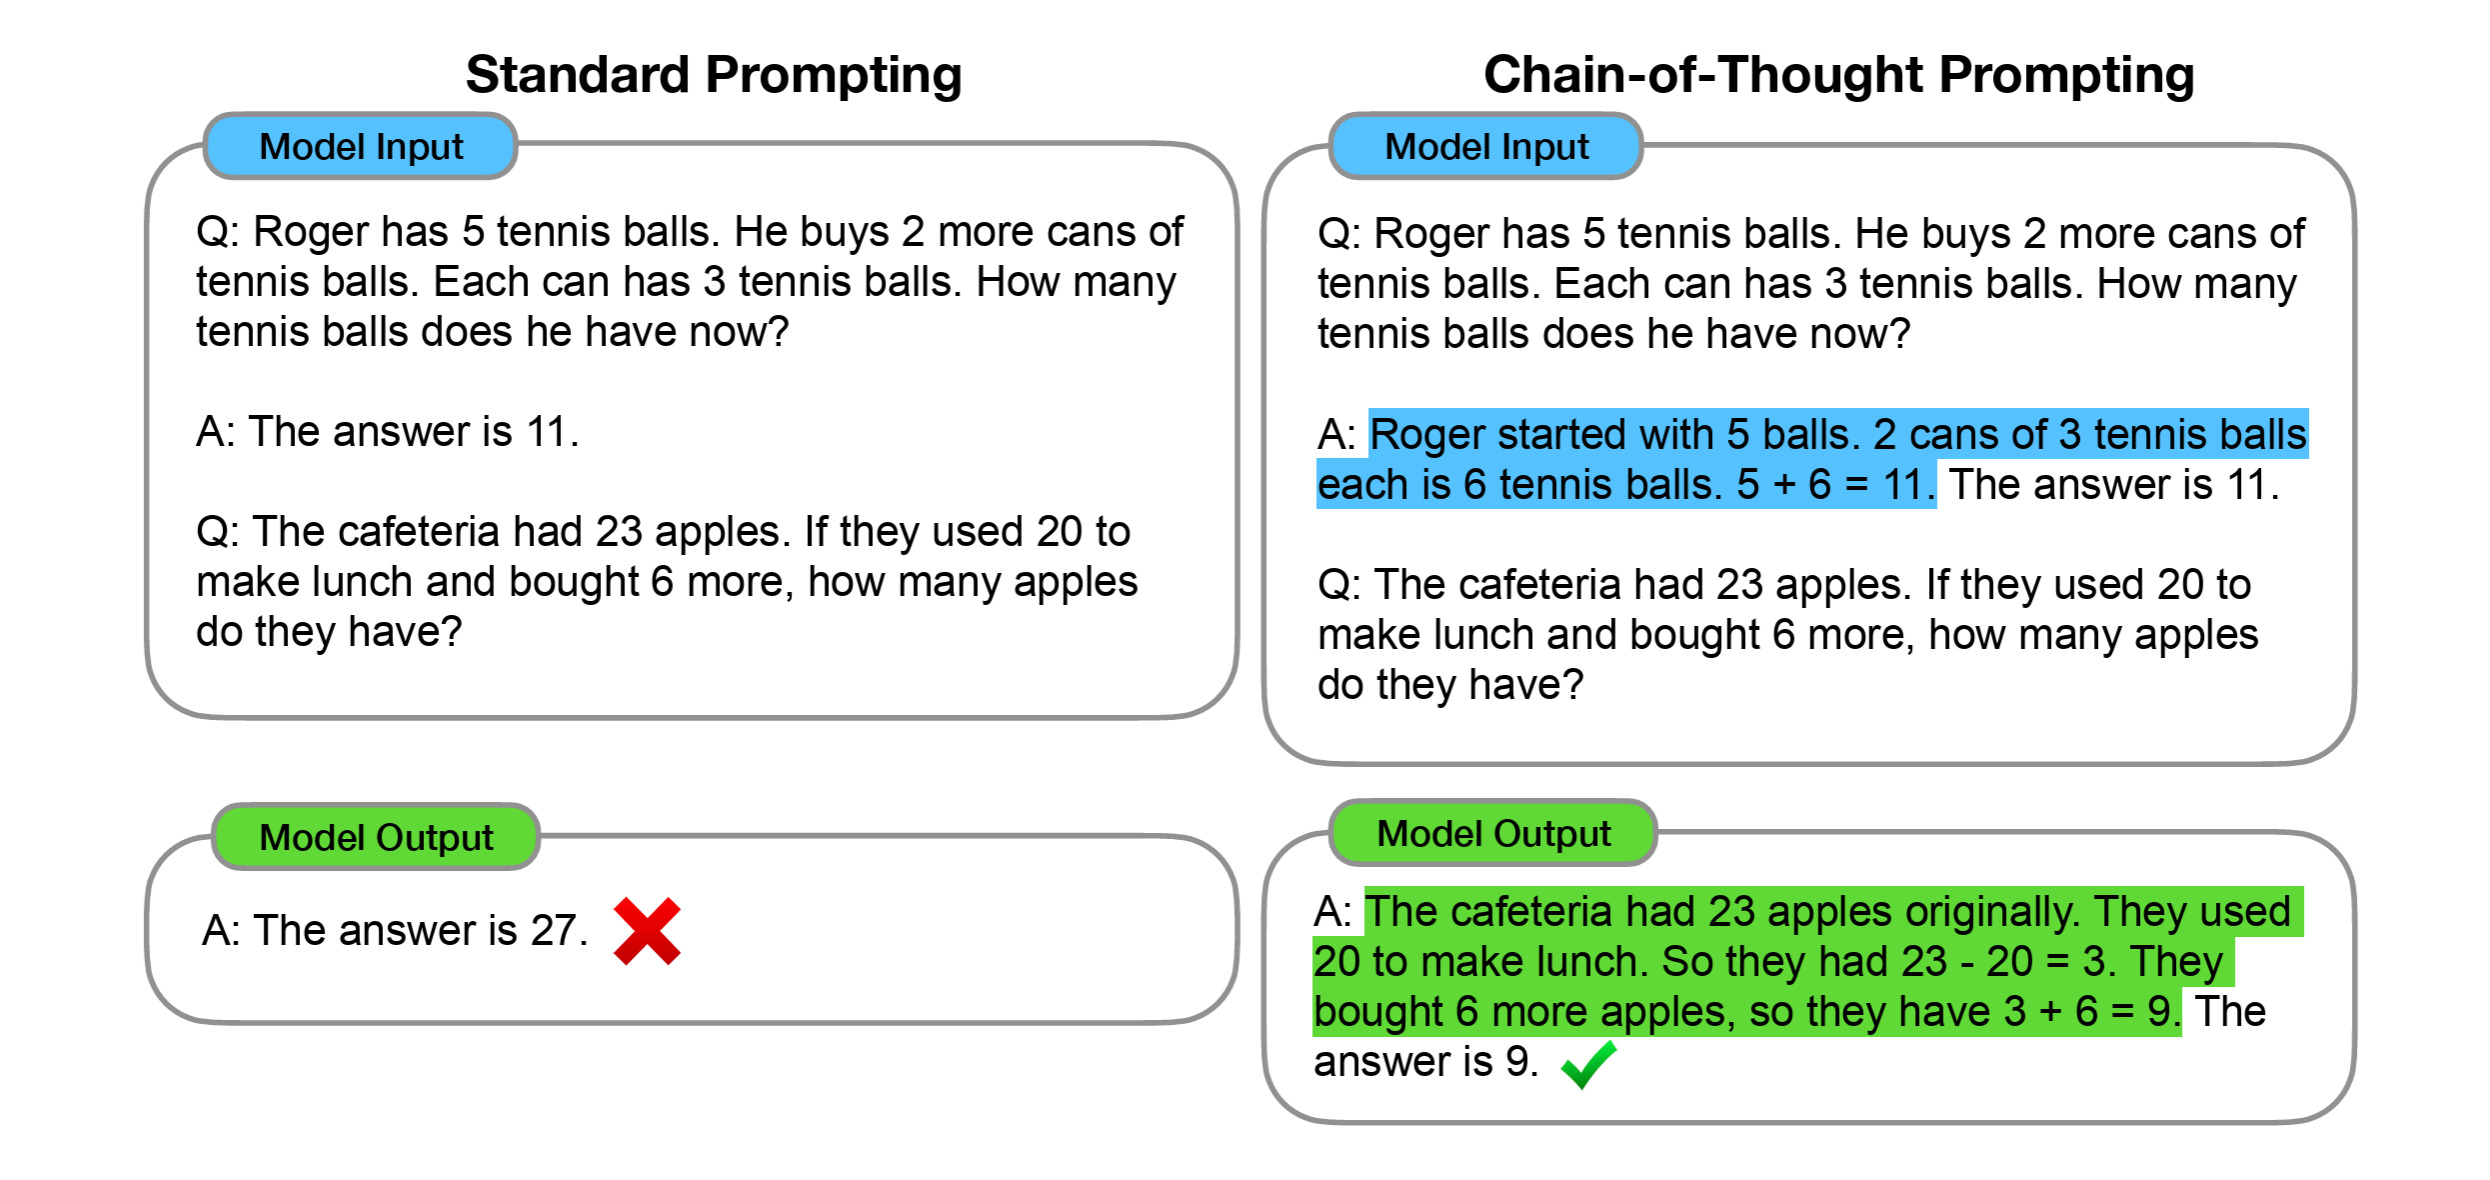
\includegraphics[width=140mm]{images/Cot}
	\caption{مثالی از روش زنجیره تفکر برای حل یک سوال از دیتاست \lr{GSM8K}}
	\label{fig_cot}
\end{figure}

\subsection{روش استدلال بدون دیدن نمونه آموزشی} 
در مقاله‌ی استدلال بدون دیدن نمونه آموزشی
\LTRfootnote{Large Language Models are Zero-Shot Reasoners} \cite{LLMzeroshot}
، پتانسیل مدل های بزرگ زبانی را برای انجام استدلال  از طریق تغییرات ساده در اعلان‌ها و بدون افزودن نمونه ای از مثال های حل شده، بررسی شده است. با اضافه کردن عبارت «بیایید مرحله به مرحله فکر کنیم» به انتهای یک اعلان، مدل‌هایی مانند GPT-3 و PaLM
\cite{palm2}
به‌طور قابل توجهی عملکرد بهتری در دیتاست‌های مختلف استدلالی ارائه می‌دهند. 
این روش بر توانایی ذاتی مدل‌ها در پردازش و تولید متن شبیه به انسان تکیه دارد و آن‌ها را تشویق می‌کند تا دنباله‌ای منطقی از تفکرات را که منجر به پاسخ نهایی می‌شود، تولید کنند. سادگی و کارآمدی این تکنیک، توانایی‌های استدلالی نهفته در مدل های بزرگ زبانی را آشکار می‌کند که می‌توان آن‌ها را بدون نیاز به آموزش وسیع و خاص برای هر وظیفه فعال کرد.
این یافته نشان می‌دهد که با مهندسی اعلان مناسب، این مدل‌ها می‌توانند طیف وسیعی از وظایف را به‌طور مؤثرتری انجام دهند و نیاز به دیتاست‌های بزرگ و برچسب‌گذاری شده و همچنین فرایندهای زمان‌بر تنظیم دقیق مدل‌ها را کاهش دهند. در شکل \ref{fig_zerocot} نمونه از حل مسئله دیتاست \lr{GSM8K} آورده شده است و جواب این روش با روش زنجیره تفکر مقایسه شده است.

\begin{figure}[!t]
	\centering
	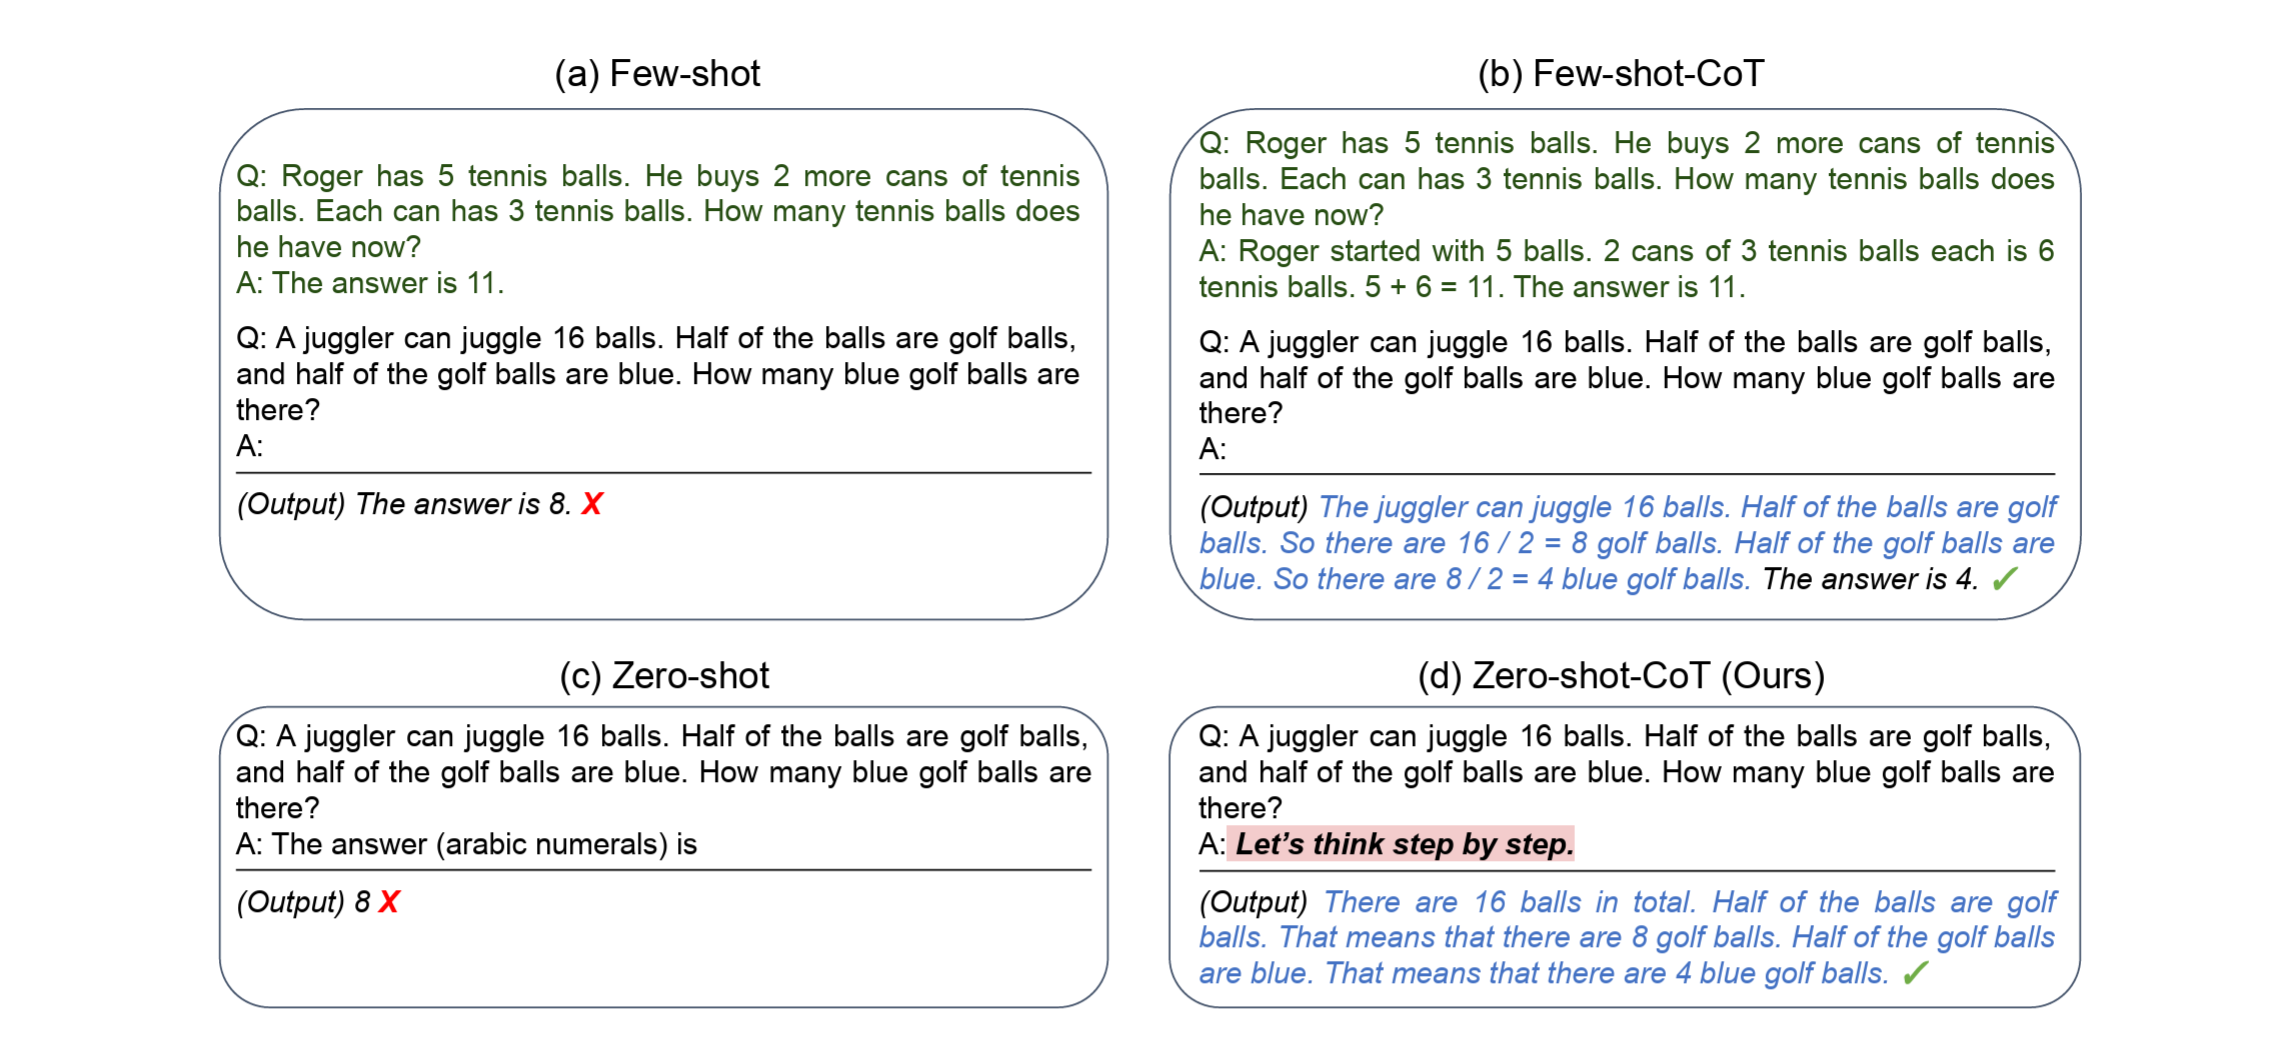
\includegraphics[width=140mm]{images/zerocot}
	\caption{مقایسه روش استدلال بدون دیدن نمونه آموزشی و روش زنجیره تفکر}
	\label{fig_zerocot}
\end{figure}


\subsection{روش برنامه تفکر}
روش برنامه تفکر
\LTRfootnote{Program-of-Thought} \cite{PoT}
یک روش پیشرفته در مهندسی اعلان است که برای بهبود توانایی‌های استدلال عددی در مدل‌های زبانی بزرگ طراحی شده است. برخلاف تکنیک زنجیره تفکر که در آن مدل هم استدلال و هم محاسبات را در قالب متن تولید می‌کرد، در برنامه تفکر این دو فرآیند از یکدیگر جدا می‌شوند. در این روش، مدل استدلال خود را به صورت کد قابل اجرایی (معمولاً با زبان‌هایی مانند پایتون) بیان می‌کند و این کد توسط یک مفسر خارجی اجرا می‌شود تا پاسخ نهایی به دست آید. این جداسازی باعث می‌شود محاسبه و استدلال از یکدیگر تفکیک شوند.

از مزایای روش برنامه تفکر می\/توان به موارد زیر اشاره کرد:
\begin{itemize}
	\item 
	با واگذاری محاسبات به یک مفسر خارجی، احتمال بروز خطاهای عددی که ممکن است در صورت انجام محاسبه و استدلال توسط خود مدل رخ دهد، کاهش می‌یابد و دقت بالاتر می\/رود.
	\item 
	مطالعات تجربی نشان داده‌اند که برنامه تفکر می‌تواند عملکرد مدل را در وظایف عددی پیچیده به طور قابل توجهی افزایش دهد. برای مثال، آزمایش‌ها نشان داده‌اند که PoT نتایجی هم‌سطح با بهترین روش‌های موجود در دیتاست‌های مسائل ریاضی و نزدیک به بهترین عملکردها در دیتاست‌های مالی داشته است.
	\item 
	نمایش مراحل استدلال به صورت کد، شفافیت فرآیند حل مسئله را افزایش می‌دهد و بررسی و درک هر مرحله را ساده‌تر می‌کند.
\end{itemize}

در شکل \ref{fig_pot} حل مسئله دنباله فیبونانچی و پیداکردن 50\/امین عضو این دنباله، با استفاده از روش زنجیره تفکر و روش برنامه تفکر بررسی شده است. به دلیل طولانی بودن مراحل حل مسئله، روش زنجیره تفکر نتوانسته جواب درست را پیدا کند ولی روش برنامه تفکر ابتدا یک کد برای حل این مسئله ارائه داده است و پس از اجرای این کد با مفسر، به جواب صحیح رسیده است.

\begin{figure}[!t]
	\centering
	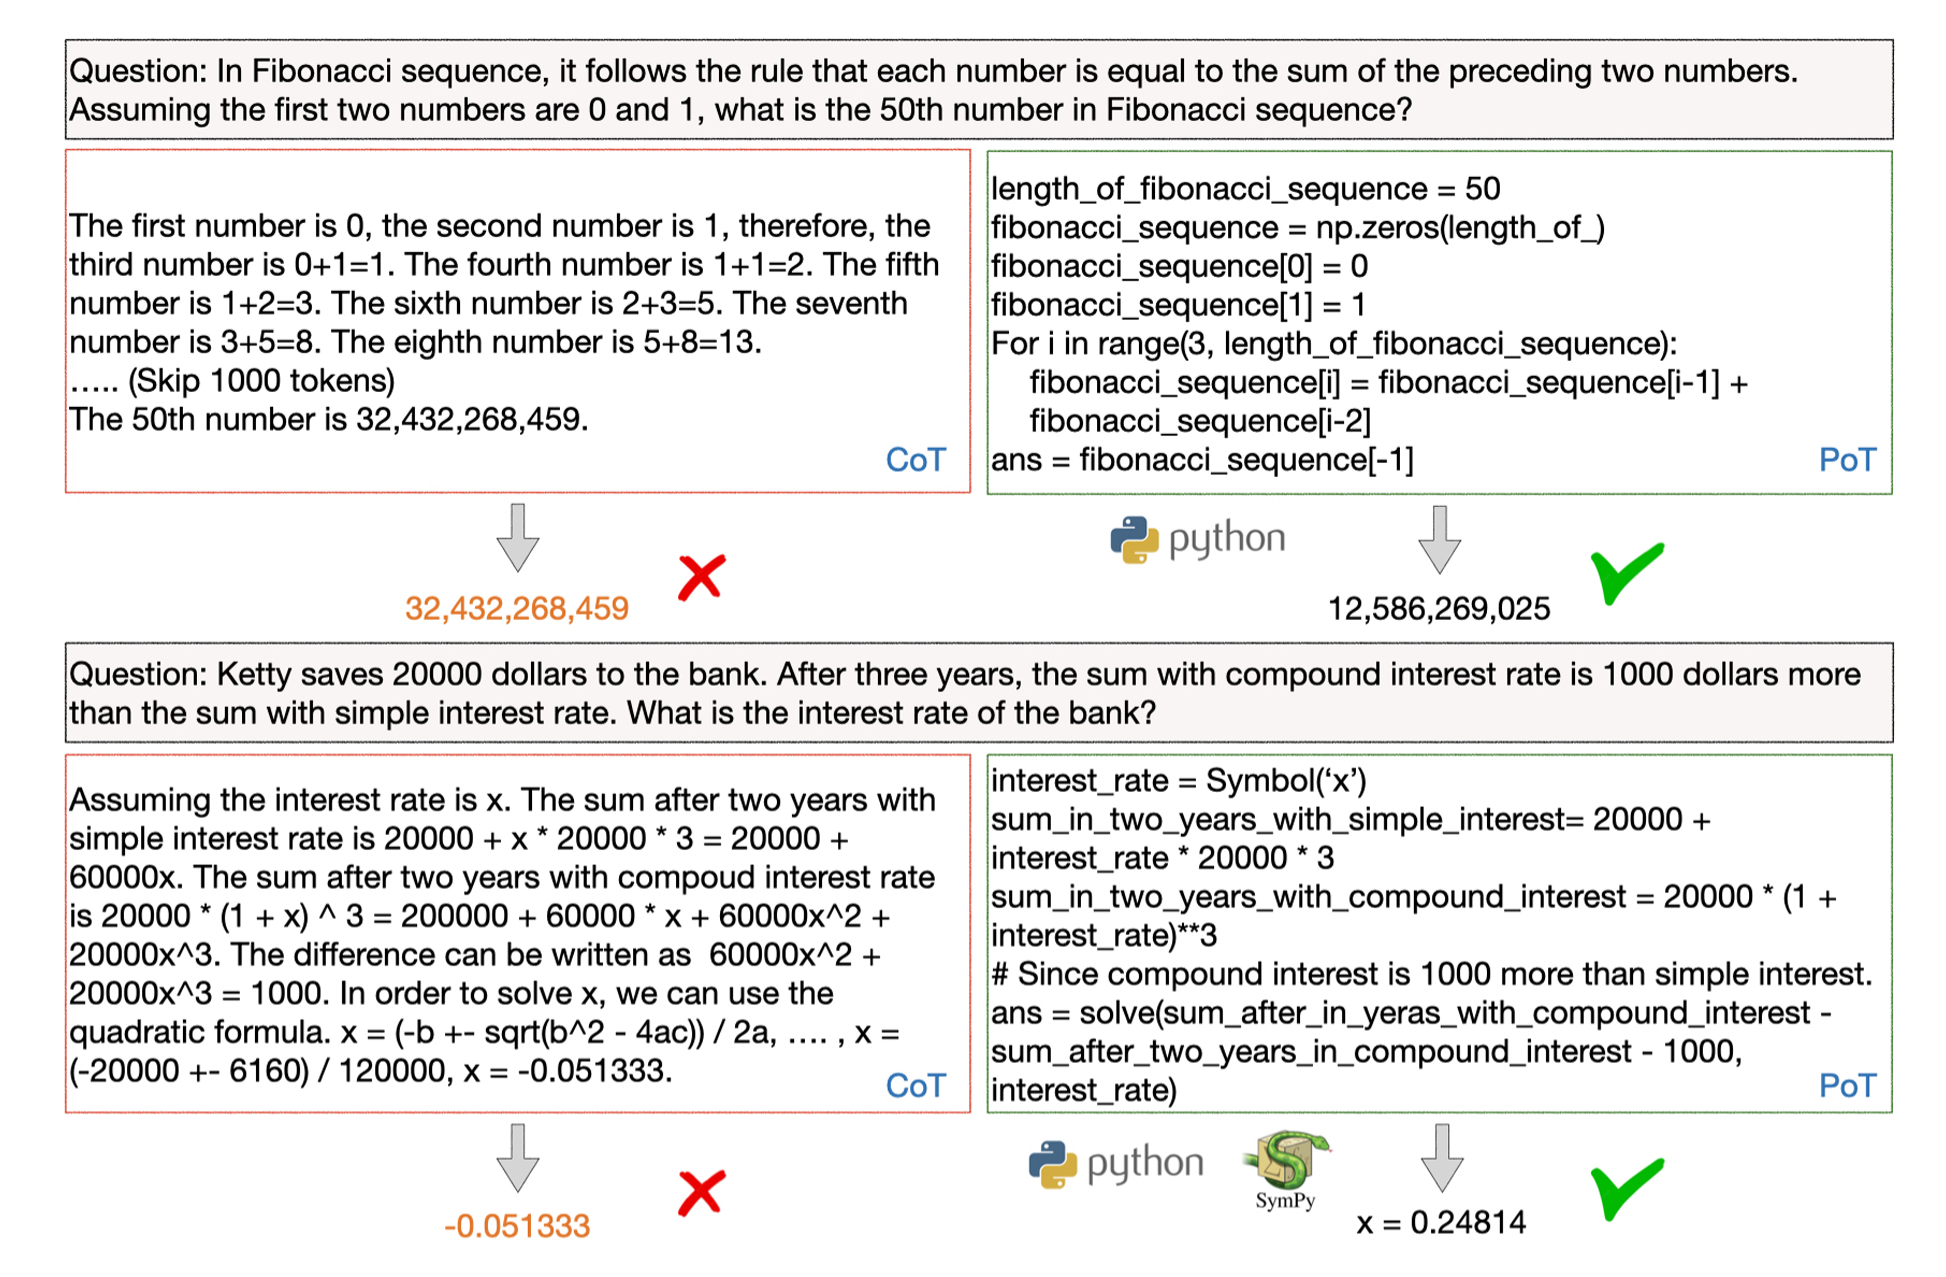
\includegraphics[width=140mm]{images/pot}
	\caption{مقایسه روش برنامه تفکر و روش زنجیره تفکر}
	\label{fig_pot}
\end{figure}

\subsection{روش بهینه سازی با اعلان}
همانطور که گفته شد مدل‌های زبانی بزرگ تا به اینجا برای وظایفی مانند تولید متن، ترجمه و خلاصه‌سازی به کار گرفته می‌شدند. با این حال، تحقیقات اخیر ظرفیت این مدل‌ها را به‌عنوان بهینه‌سازها مورد بررسی قرار داده‌اند و از قابلیت‌های استدلالی آن‌ها برای حل مسائل پیچیده بهینه‌سازی بهره برده‌اند.

یکی از رویکردهای برجسته در این زمینه، روش بهینه سازی با اعلان 
\LTRfootnote{Optimization by PROmpting} \cite{opro}
 است. این روش از مدل‌های زبانی بزرگ برای تولید راه‌حل‌های مسائل بهینه‌سازی بر اساس اعلان‌های زبان طبیعی استفاده می‌کند. این فرآیند شامل تکرارهای پی‌در‌پی است که در آن، اعلان جدید با راه‌حل‌ها و ارزیابی‌های قبلی طراحی می‌شود و در تکرارهای بعدی، راه‌حل‌های بهتری پیشنهاد می‌دهد. این روش در کاربردهای مختلفی همچون رگرسیون خطی
 \LTRfootnote{Linear Regression}
 ، مسئله فروشنده دوره‌گرد
 \LTRfootnote{Traveling Salesman Problem}
  و حتی بهینه‌سازی اعلان برای خود مدل‌های زبانی بزرگ مؤثر واقع شده است. جالب توجه اینکه این روش توانسته تا ۸٪ بهبود عملکرد در دیتاست \lr{GSM8K} و تا ۵۰٪ بهبود در وظایف دشوار
  \LTRfootnote{Big-Bench Hard}
   داشته باشد و حتی از اعلان‌های طراحی‌شده توسط انسان نیز پیشی بگیرد.

در روش بهینه سازی با اعلان، مسئله بهینه‌سازی با زبان طبیعی توصیف می‌شود تا مدل بتواند بافت و هدف مسئله را درک کند. همانطور که در شکل \ref{fig_opro} در هر مرحله از بهینه‌سازی، مدل با توجه به اعلان شامل راه‌حل‌ها و ارزیابی‌های قبلی، راه‌حل‌های جدیدی تولید می‌کند. این راه‌حل‌ها ارزیابی شده و سپس برای تکرار بعدی در اعلان گنجانده می‌شوند و این چرخه بهبود مستمر ادامه پیدا می‌کند.

\begin{figure}[!t]
	\centering
	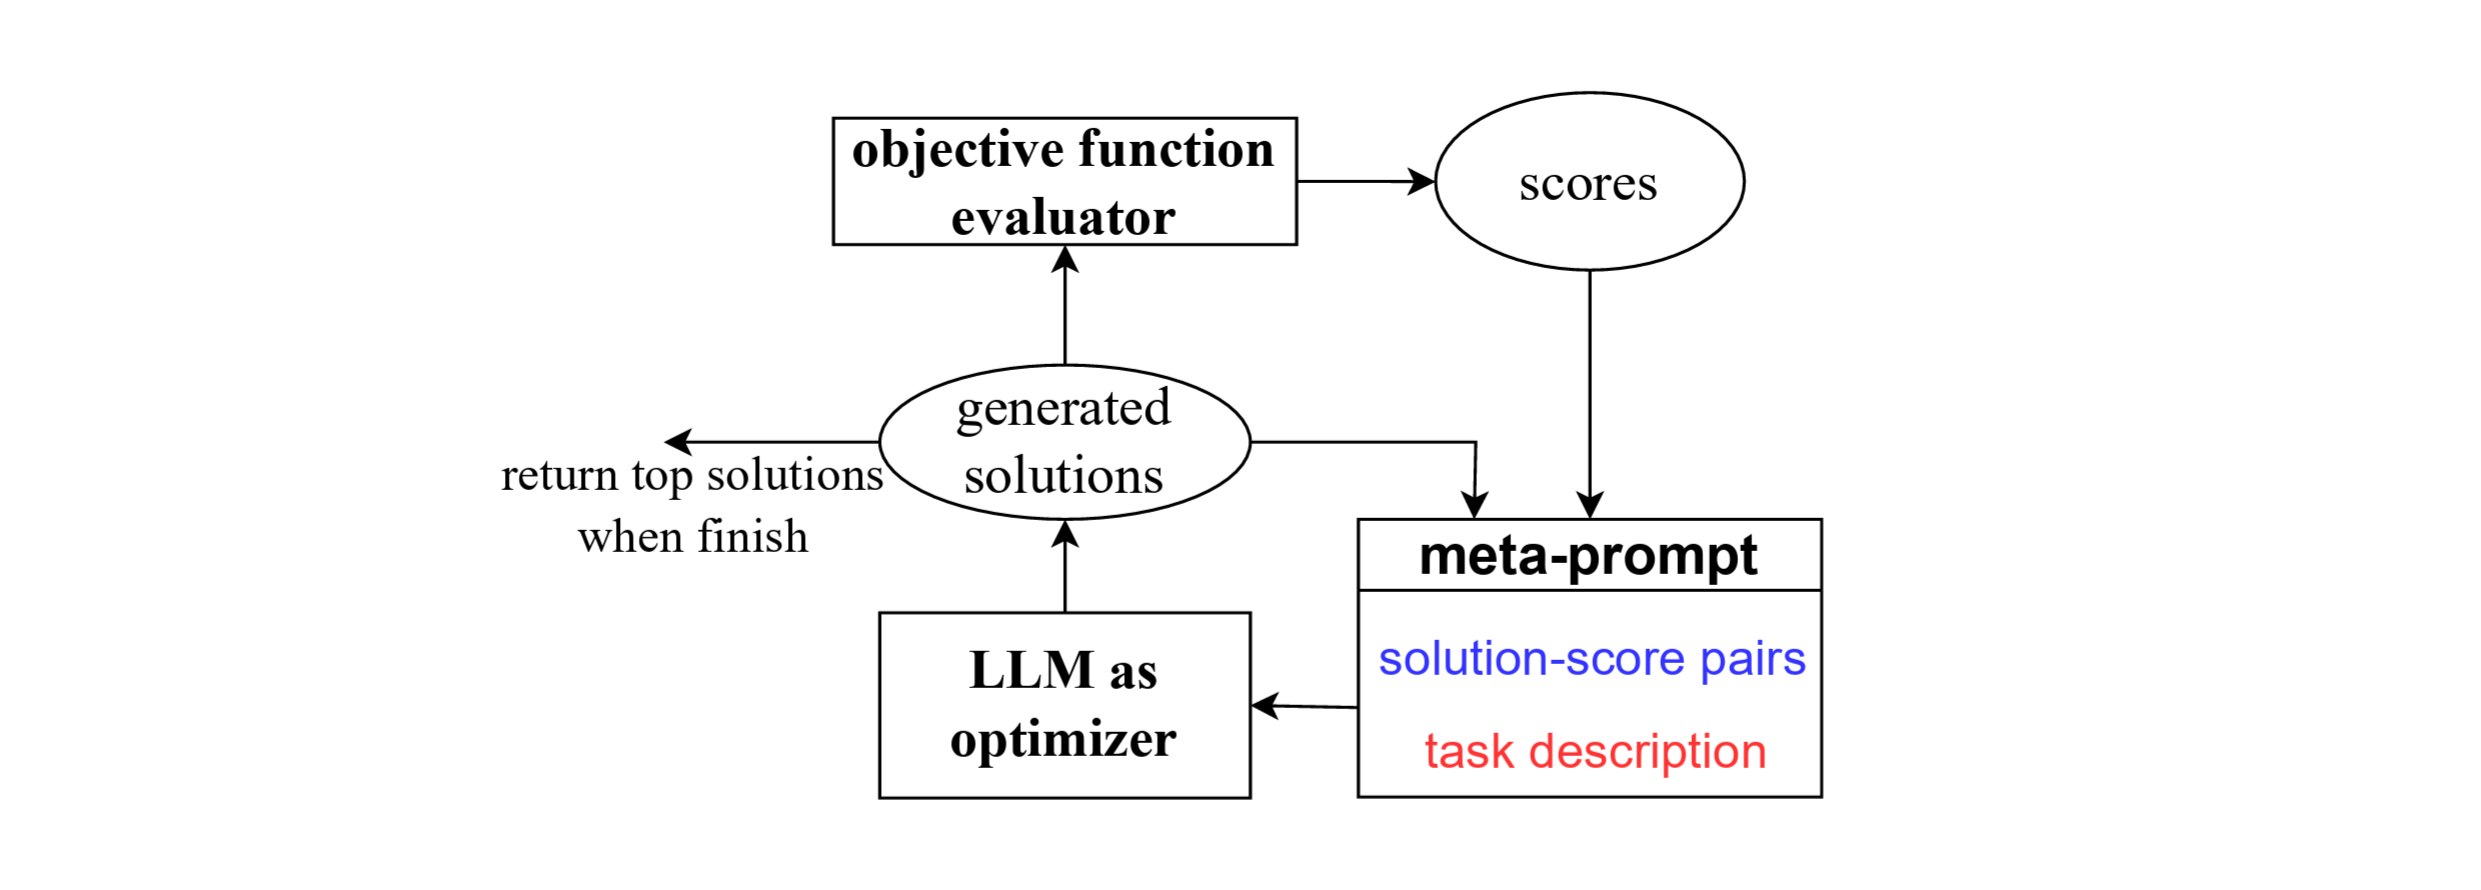
\includegraphics[width=140mm]{images/opro}
	\caption{دیاگرام روش بهینه سازی با اعلان}
	\label{fig_opro}
\end{figure}


از مزایای استفاده از مدل‌های زبانی بزرگ به‌عنوان بهینه‌ساز می\/توان به موارد زیر اشاره کرد:

\begin{itemize}
	\item 
	مدل‌های زبانی بزرگ به دلیل توانایی درک و تولید متنی مشابه انسان، می‌توانند به انواع مختلف مسائل بهینه‌سازی که با زبان طبیعی توصیف می‌شوند، پاسخ دهند.
	\item 
	همچنین این مدل ها قادر به انجام بهینه‌سازی در مسائلی هستند که اطلاعات گرادیان در دسترس نیست یا به‌دست‌آوردن آن دشوار است و به همین دلیل رویکردی بدون نیاز به مشتق ارائه می‌دهند.
	\item 
	از طرفی این مدل ها می‌توانند اعلان‌های خود را بهینه کنند و بدون نیاز به آموزش مجدد، عملکرد خود را در وظایف خاص بهبود دهند.
\end{itemize}




\subsection{روش برنامه\/ریزی و حل}
روش برنامه\/ریزی و حل
\LTRfootnote{Plan-and-Solve (PS)}
یک تکنیک پیشرفته در مهندسی اعلان است که بهبود عملکرد مدل‌های زبانی بزرگ را در حل مسائل پیچیده مورد هدف قرار می‌دهد. در این روش، مدل ابتدا یک برنامه‌ریزی
\LTRfootnote{Planing}
 انجام داده و سپس بر اساس آن، به حل مسئله
\LTRfootnote{Solve}
  می‌پردازد.  

برخلاف روش‌های سنتی که مدل را مستقیماً درگیر حل مسئله می‌کنند، این روش باعث کاهش نرخ خطا شده و دقت پاسخ‌های مدل را افزایش می‌دهد. روش برنامه ریزی و حل به‌ویژه در مسائلی که نیاز به چندین مرحله استدلالی دارند، مانند حل مسائل ریاضی، تحلیل منطقی و برنامه‌ریزی وظایف، بسیار کارآمد است.  


این روش شامل دو مرحله اصلی است:  

\begin{enumerate}
	\item برنامه‌ریزی 
	\LTRfootnote{Plan Phase}:
	مدل یک برنامه کلی برای حل مسئله ارائه می‌دهد، شامل مراحل موردنیاز برای رسیدن به پاسخ.  
	\item حل مسئله
	\LTRfootnote{Solve Phase}:
	مدل بر اساس برنامه تولیدشده، گام‌به‌گام راه‌حل را پیاده‌سازی کرده و پاسخ نهایی را استخراج می‌کند.  
\end{enumerate}  

این تفکیک دو مرحله‌ای، عملکرد مدل را بهبود می‌بخشد زیرا ابتدا ساختار حل مسئله مشخص شده و سپس محاسبات انجام می‌شود.  
در ادامه یک مسئله و راه حل این روش برای آن مسئله را بررسی می\/کنیم.

مسئله:	سن علی ۳ برابر سن برادرش است. ۴ سال پیش، مجموع سن آن‌ها ۲۰ سال بوده است. سن هر یک را مشخص کنید. 

\begin{enumerate}
	\item اجرای مرحله برنامه‌ریزی:
	\begin{itemize}
		\item تعریف متغیرها: فرض کنیم سن برادر علی را $X$ در نظر بگیریم.  
		\item رابطه کنونی: سن علی برابر با $3X$ است.  
		\item رابطه در گذشته: ۴ سال پیش، سن برادر علی برابر $X-4$ و سن علی برابر $3X-4$ بوده است.  
		\item معادله کلی:  
		\[
		(X - 4) + (3X - 4) = 20
		\]
		\item حل معادله و یافتن مقدار $X$
	\end{itemize} 
	
	\item اجرای مرحله حل:
	\[
	X - 4 + 3X - 4 = 20
	\]  
	\[
	4X - 8 = 20
	\]  
	\[
	4X = 28
	\]  
	\[
	X = 7
	\]  
	در نتیجه :  
	\begin{itemize}
		\item سن برادر علی : $7$ سال  
		\item سن علی : $3 \times 7 = 21$ سال  
	\end{itemize}  
\end{enumerate}

با بررسی این مثال می\/توان متوجه افزایش دقت حل مسائل چند مرحله ای با استفاده از روش برنامه ریزی و حل شد و همچنین عملکرد برنامه ریزی و سپس عمل را مشاهده کرد که مشابه سیستم تفکر انسانی است.
در شکل \ref{fig_ps} یک مثال دیگر از این روش آورده شده است.

\begin{figure}[!t]
	\centering
	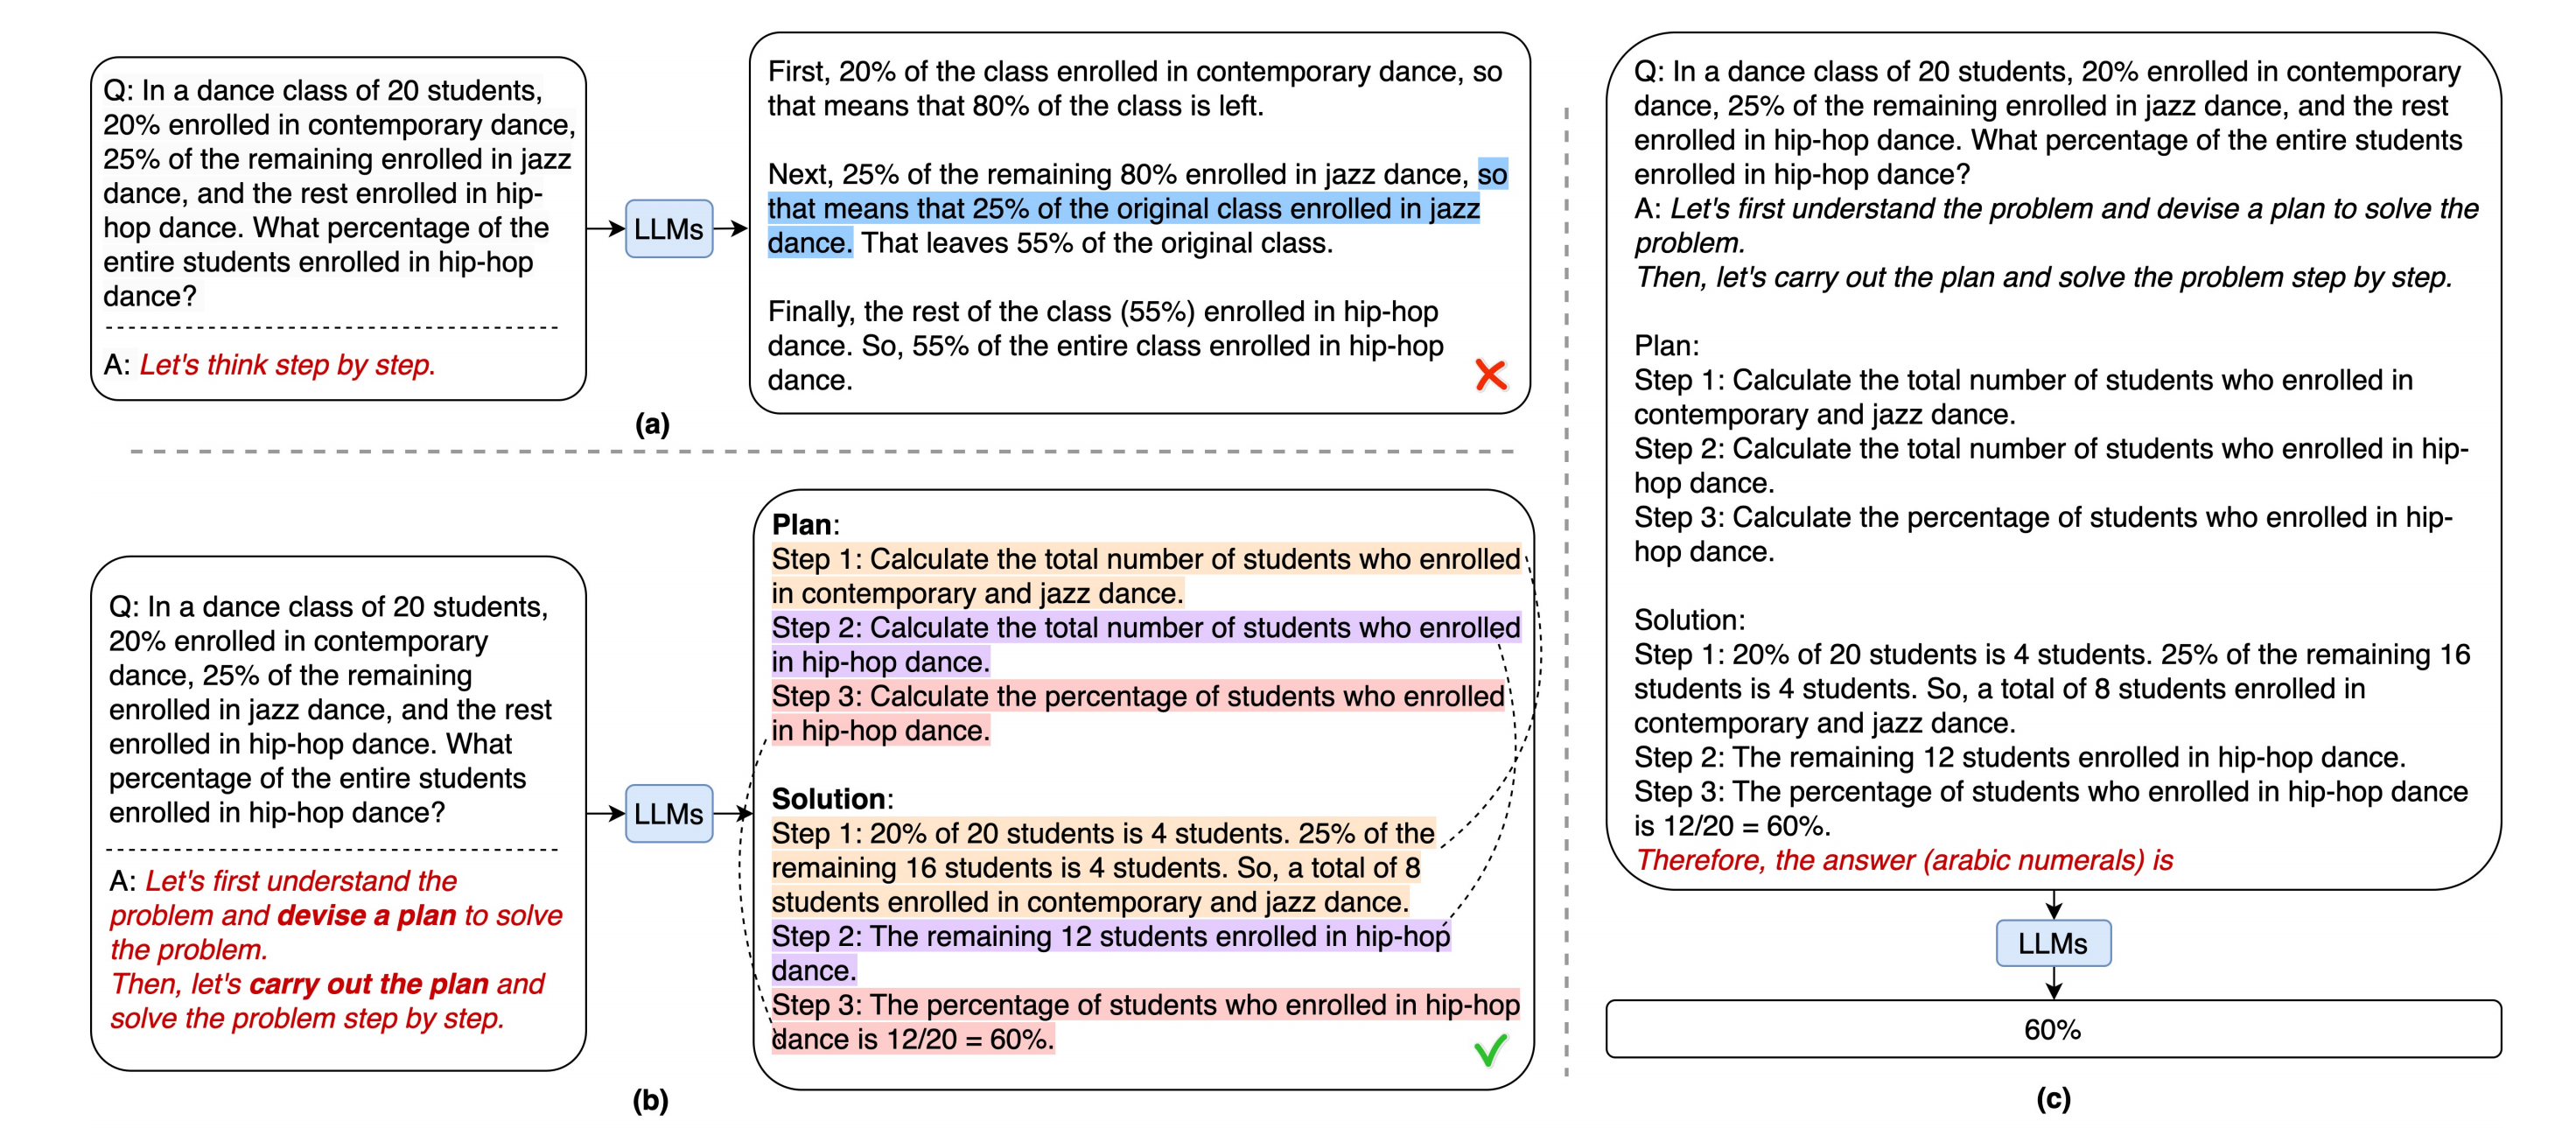
\includegraphics[width=160mm]{images/ps}
	\caption{یک مثال از روش برنامه\/ریزی و حل}
	\label{fig_ps}
\end{figure}


\section{بهینه‌سازی خودکار اعلان‌ها}
بهینه‌سازی خودکار اعلان‌ها یک رویکرد نوین در مهندسی اعلان است که با بهره‌گیری از الگوریتم‌های جستجو و بهینه‌سازی، به صورت سیستماتیک بهترین ورودی‌های متنی را برای مدل‌های زبانی شناسایی و تولید می‌کند. در این روش به جای تکیه بر شهود انسانی و روش‌های آزمون و خطا، از تکنیک‌هایی مانند الگوریتم‌های تکاملی، جستجوی تصادفی و یادگیری تقویتی استفاده می‌شود. این الگوریتم‌ها فضای اعلان‌ها را مورد بررسی قرار داده و بر اساس معیارهای مشخصی مانند دقت، انسجام و ارتباط معنایی، به انتخاب بهینه‌ترین اعلان‌ها می‌پردازند.

یکی از مزایای مهم بهینه‌سازی خودکار اعلان‌ها این است که در مقیاس‌های بزرگ و در زمان‌های کوتاه، قادر به دستیابی به نتایج بهینه می‌باشد. بهینه‌سازی خودکار پرامت ها با ارائه چارچوبی سیستماتیک، امکان ارزیابی سریع و انتخاب اعلان‌های بهینه را فراهم می‌آورد. این دو رویکرد می‌توانند مکمل یکدیگر عمل کرده و در کاربردهایی که نیاز به سرعت و دقت بالا دارند، مانند پردازش دسته‌جمعی داده‌های متنی یا تنظیم خودکار اعلان‌ها برای وظایف متنوع، عملکرد بهتری ارائه دهند.

\subsection{روش زنجیره تفکر خودکار}
از اولین جرقه های خودکارسازی مهندسی اعلان، میتوان به خودکارسازی تولید زنجیره‌های استدلالی در روش زنجیره تفکر اشاره کرد. روش زنجیره تفکر خودکار 
\LTRfootnote{AUTOMATIC CHAIN-OF-THOUGHT PROMPTING (Auto-CoT)} \cite{auto_cot}
 به‌طور خودکار زنجیره‌هایی از استدلال‌ها و سوالات را برای ساخت نسخهها ایجاد می‌کند. این روش شامل دو مرحله اصلی است. مرحله اول خوشه‌بندی سوالات و تقسیم سوالات یک مجموعه‌داده به چندین خوشه و مرحله دوم نمونه‌گیری از نسخهها و انتخاب یک سوال نماینده از هر خوشه و تولید زنجیره استدلال برای آن است. روند کلی این روش در شکل \ref{fig_autocot} نشان داده شده است.

در مرحله اول، از آنجایی که خوشه‌بندی مبتنی بر تنوع می‌تواند از گمراهی ناشی از شباهت جلوگیری کند، این روش تحلیل خوشه‌ای را برای مجموعه‌ای از سوالات $Q$ انجام می‌دهد. بدین صورت که ابتدا برای هر سوال در $Q$، یک بردار نمایشی با استفاده از \lr{Sentence-BERT} \cite{sentenceBert} محاسبه می\/شود و سپس این بردارهای متنی میانگین‌گیری شده و یک بردار با اندازه ثابت برای هر سوال ایجاد می‌شود. پس از آن، با استفاده از الگوریتم خوشه‌بندی k-means ، سوالات به $k$ خوشه تقسیم می‌شوند. در نهایت برای هر خوشه $i$، سوالات آن خوشه را به‌صورت یک لیست مرتب‌شده \lr{$q^{(i)} = [q^{(i)}_1, q^{(i)}_2, \ldots]$} بر اساس فاصله از مرکز خوشه به ترتیب صعودی مرتب می‌شوند.

در مرحله دوم، برای سوالات نمونه‌گیری‌شده، زنجیره‌های استدلال تولید می\/شوند و نسخههایی که با معیارهای انتخاب مطابقت دارند استخراج می\/شوند. به‌طور دقیق‌تر، برای هر خوشه $i$، یک نسخه به صورت \lr{$d^{(i)}$} (ترکیبی از سوال، استدلال و پاسخ) ساخته می\/شود. برای خوشه $i$، سوالات مرتب‌شده در لیست \lr{$q^{(i)} = [q^{(i)}_1, q^{(i)}_2, \ldots]$} تا زمانی که معیارهای انتخاب برآورده شوند، بررسی می‌شوند.

به عبارت دیگر، سوالی که به مرکز خوشه نزدیک‌تر است، زودتر بررسی می‌شود. فرض کنید سوال \lr{$q^{(i)}_j$} که $j$-اُمین سوال نزدیک به مرکز خوشه $i$ است، در حال بررسی باشد. یک ورودی به شکل زیر ساخته می‌شود:

\begin{center}
	\lr{[Q: $q^{(i)}_j$ A: [P]]}
\end{center}

سپس یک نسخه کاندید برای خوشه $i$ به صورت زیر ساخته می‌شود:

\begin{center}
	\lr{[Q: $q^{(i)}_j$ A: $r^{(i)}_j$ $a^{(i)}_j$]}
\end{center}

مشابه معیارهای مورد استفاده در نسخه\/های دستی روش زنجیره تفکر \cite{CoT}, معیار انتخاب این الگوریتم نیز بر قوانین ساده‌ای تکیه دارد تا سوالات و استدلال‌های ساده‌تر را انتخاب کند: نسخه \lr{$d^{(i)}$} به‌عنوان \lr{$d^{(i)}_j$} انتخاب می‌شود اگر سوال \lr{$q^{(i)}_j$} دارای کمتر از ۶۰ توکن و استدلال \lr{$r^{(i)}_j$} دارای کمتر از ۵ گام استدلالی باشد.

\begin{figure}[!t]
	\centering
	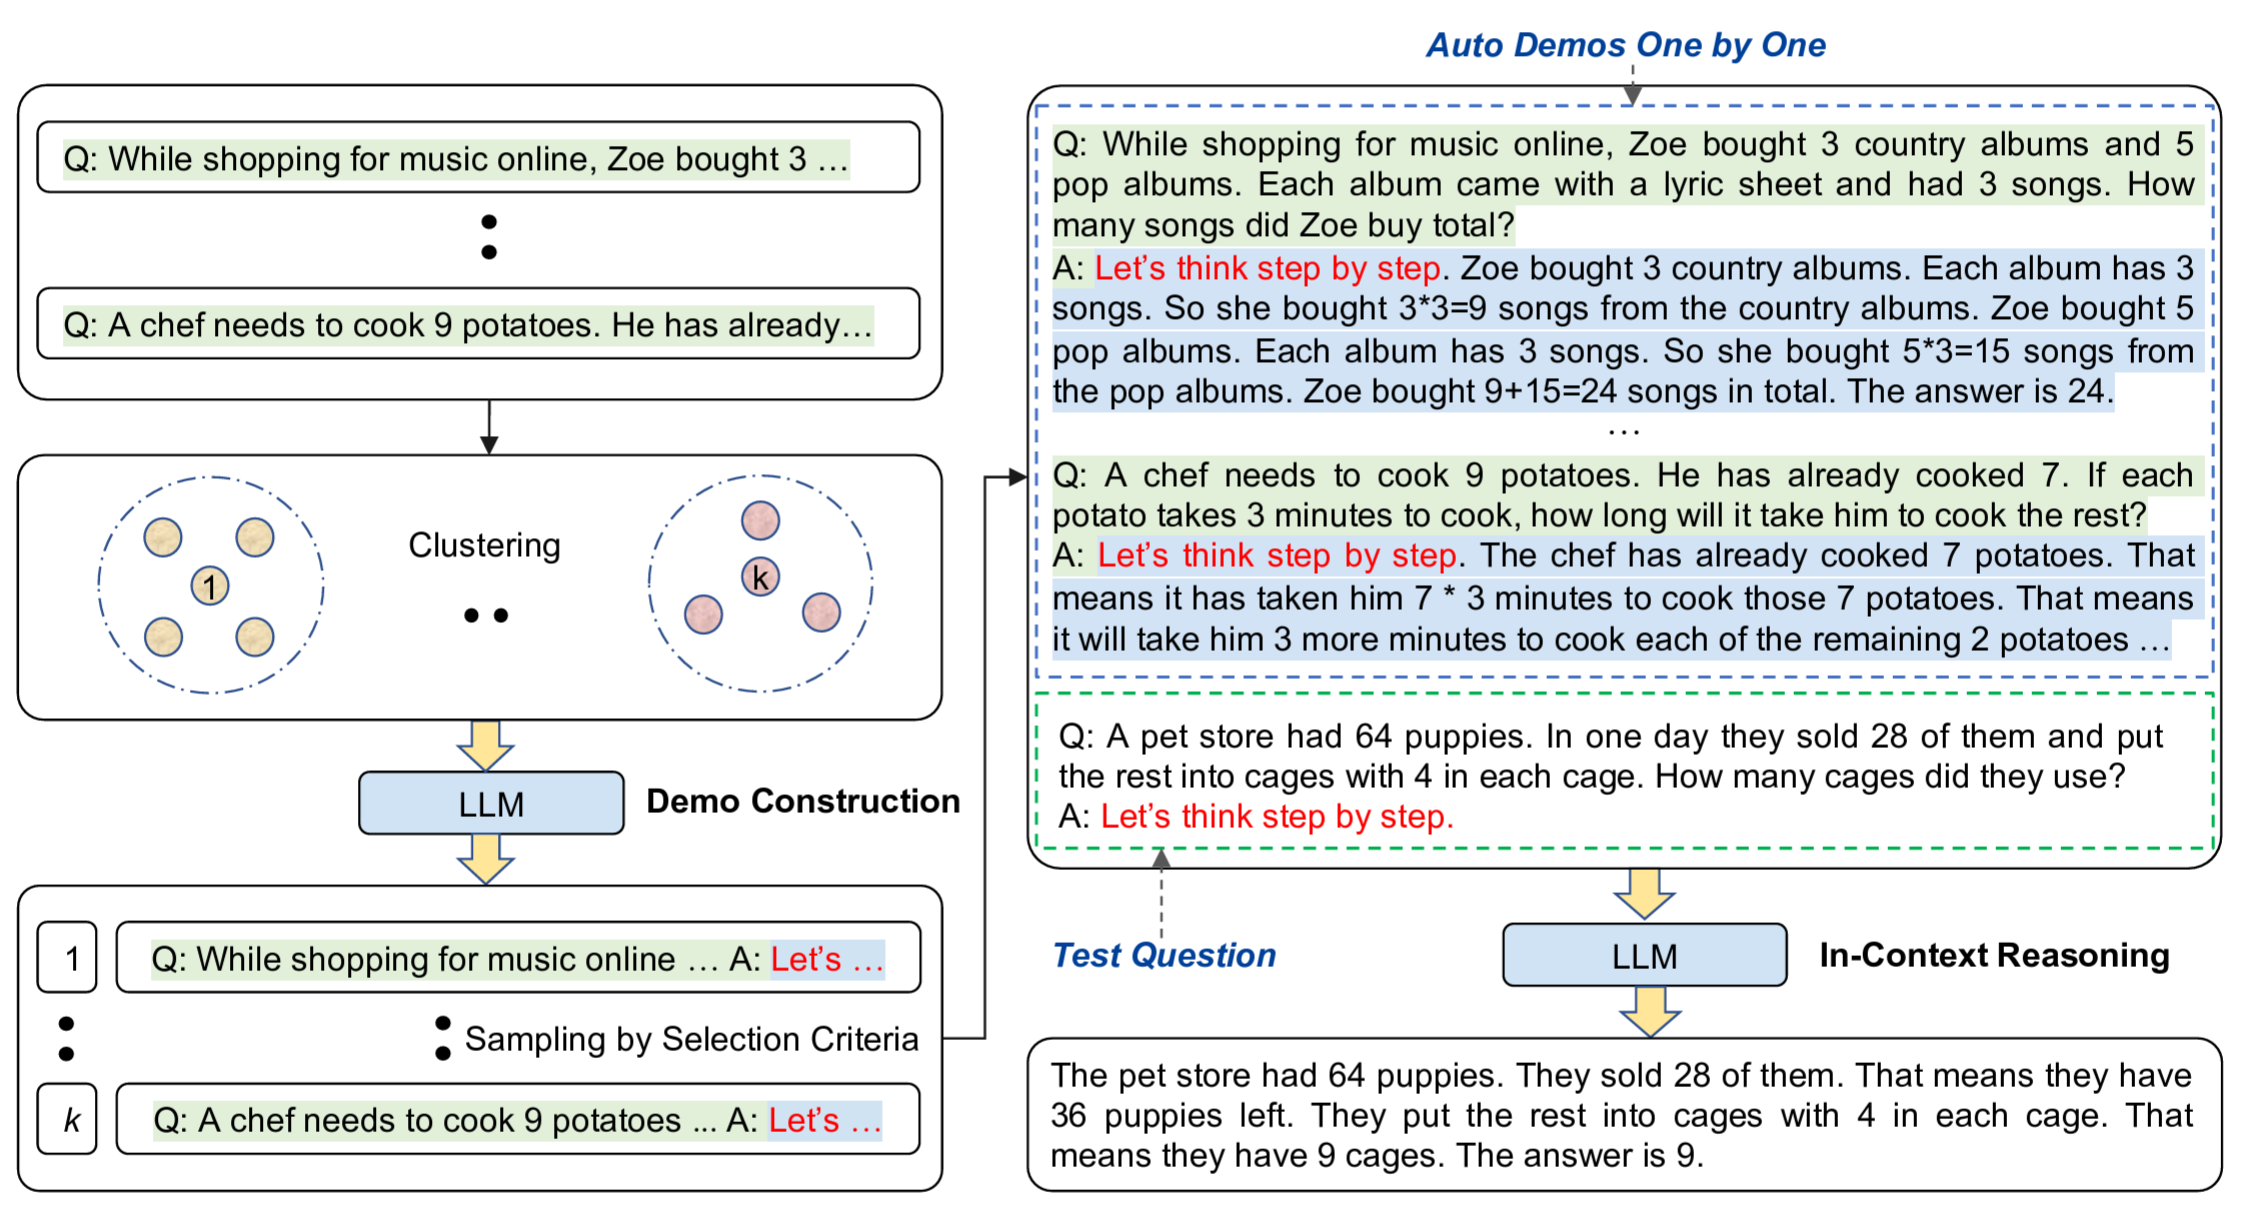
\includegraphics[width=140mm]{images/autocot}
	\caption{دیاگرام روش auto-CoT}
	\label{fig_autocot}
\end{figure}

\subsection{روش مهندس اعلان خودکار}
روش  مهندس اعلان خودکار
\LTRfootnote{Auto Prompt Engineer} \cite{APE}
 از خود مدل‌های زبانی بزرگ برای خودکارسازی فرآیند ایجاد و بهینه‌سازی اعلان‌ها استفاده می‌کند. در این روش، یک مدل زبانی، مجموعه‌ای از اعلان‌های مختلف تولید می‌کند و سپس این اعلان‌ها بر اساس کیفیت پاسخ‌هایی که از یک مدل دیگر دریافت می‌شود، ارزیابی می‌شوند. این فرآیند به‌صورت تکراری ادامه می‌یابد تا مؤثرترین اعلان‌ها شناسایی شوند. نتایج در ۲۴ وظیفه مختلف در حوزه پردازش زبان طبیعی نشان داده که اعلان‌های تولید شده توسط این روش در اغلب موارد عملکرد بهتری نسبت به روش‌های قبلی داشته‌اند و در ۱۹ مورد از ۲۴ وظیفه، کیفیتی معادل یا نزدیک به اعلان‌های طراحی شده توسط انسان ارائه کرده‌اند.

تأثیرات این روش قابل توجه است؛ این روش نیاز به مهندسان اعلان انسانی را کاهش می‌دهد، فرآیند توسعه را سریع‌تر می‌کند و سازگاری مدل‌های زبانی بزرگ با وظایف مختلف را افزایش می‌دهد. این پیشرفت نشان‌دهنده ظرفیت مدل‌های بزرگ زبانی برای نه‌تنها انجام وظایف، بلکه بهینه‌سازی دستورالعمل‌های خودشان نیز هست و گامی مهم به سوی سامانه‌های هوشمند خودمختارتر به‌شمار می‌رود.

\subsection{روش مولد اعلان}
روش مولد اعلان
\LTRfootnote{Promptbreeder} \cite{PromptBreeder}
 یک سیستم خودارجاعی
 \LTRfootnote{self-referential}
  و تکاملی برای بهبود خودکار اعلان‌های مورد استفاده در مدل‌های زبانی بزرگ است. این روش با الهام از الگوریتم‌های تکاملی و فرآیندهای خودبهبوددهی
  \LTRfootnote{self-improvment}
  ، به جای اتکا بر اعلان‌های دستی و مهندسی‌شده، به طور خودکار اعلان‌هایی را تولید و اصلاح می‌کند که می‌توانند عملکرد مدل را در حل مسائل مختلف بهبود بخشند. ویژگی کلیدی این روش این است که نه‌تنها اعلان‌های وظیفه
  \LTRfootnote{Task Prompts}
   را تکامل می‌دهد، بلکه اعلان‌های تغییر
   \LTRfootnote{Mutation Prompts}
    را نیز که برای تغییر اعلان‌های مورد جستجو استفاده می‌شوند، بهبود می‌بخشد.  

این الگوریتم از یک فرآیند تکاملی مبتنی بر جمعیت
\LTRfootnote{population base}
 استفاده می‌کند. همانطور که در شکل \ref{fig_promptbreeder} نشان داده شده است، در ابتدا یک مجموعه از اعلان‌های اولیه به همراه دستورات تغییر تولید می‌شود. سپس، در هر نسل از فرآیند تکامل: 
 \begin{enumerate}
 	\item ارزیابی سازگاری
 	\LTRfootnote{Fitness Evaluation}: اعلان‌ها بر اساس عملکردشان در پاسخ‌دهی به مجموعه‌ای از سؤالات آموزشی ارزیابی می‌شوند.
 	
 	\item انتخاب
 	\LTRfootnote{Selection}: دو اعلان به‌صورت تصادفی انتخاب شده و مقایسه می‌شوند؛ اعلانی که عملکرد بهتری داشته باشد، انتخاب می‌شود.
 	
 	\item اعمال تغییرات
 	\LTRfootnote{Mutation}: اعلان انتخاب‌شده با استفاده از عملگرهای تکاملی تغییر داده می‌شود. این تغییرات شامل تولید نسخه‌های جدید از اعلان، اصلاح بر اساس الگوهای موفق، و یا حتی بهبود خود دستور تغییر است.  
 	
 	\item جایگزینی
 	\LTRfootnote{Replacement}: نسخه‌ی بهبودیافته جایگزین اعلان با عملکرد ضعیف‌تر شده و این فرآیند در نسل‌های بعدی تکرار می‌شود.
 \end{enumerate} 

عملگرهای تکاملی شامل جهش مستقیم
\LTRfootnote{Direct Mutation}
، جهش مبتنی بر توزیع
\LTRfootnote{Estimation of Distribution (EDA) Mutation}
، ابرجهش
\LTRfootnote{Hypermutation}
، جهش لامارکین
\LTRfootnote{Lamarckian Mutation}
، و ترکیب اعلان‌ها
\LTRfootnote{Prompt Crossover and Context Shuffling}
 هستند که هر یک روش‌های متفاوتی را برای اصلاح و بهبود اعلان‌ها ارائه می‌دهند. با ادامه این فرآیند در طی چندین نسل، اعلان‌ها به تدریج بهینه شده و به عملکرد بهتری در مدل‌های زبانی منجر می‌شوند.  
 
\begin{figure}[!t]
	\centering
	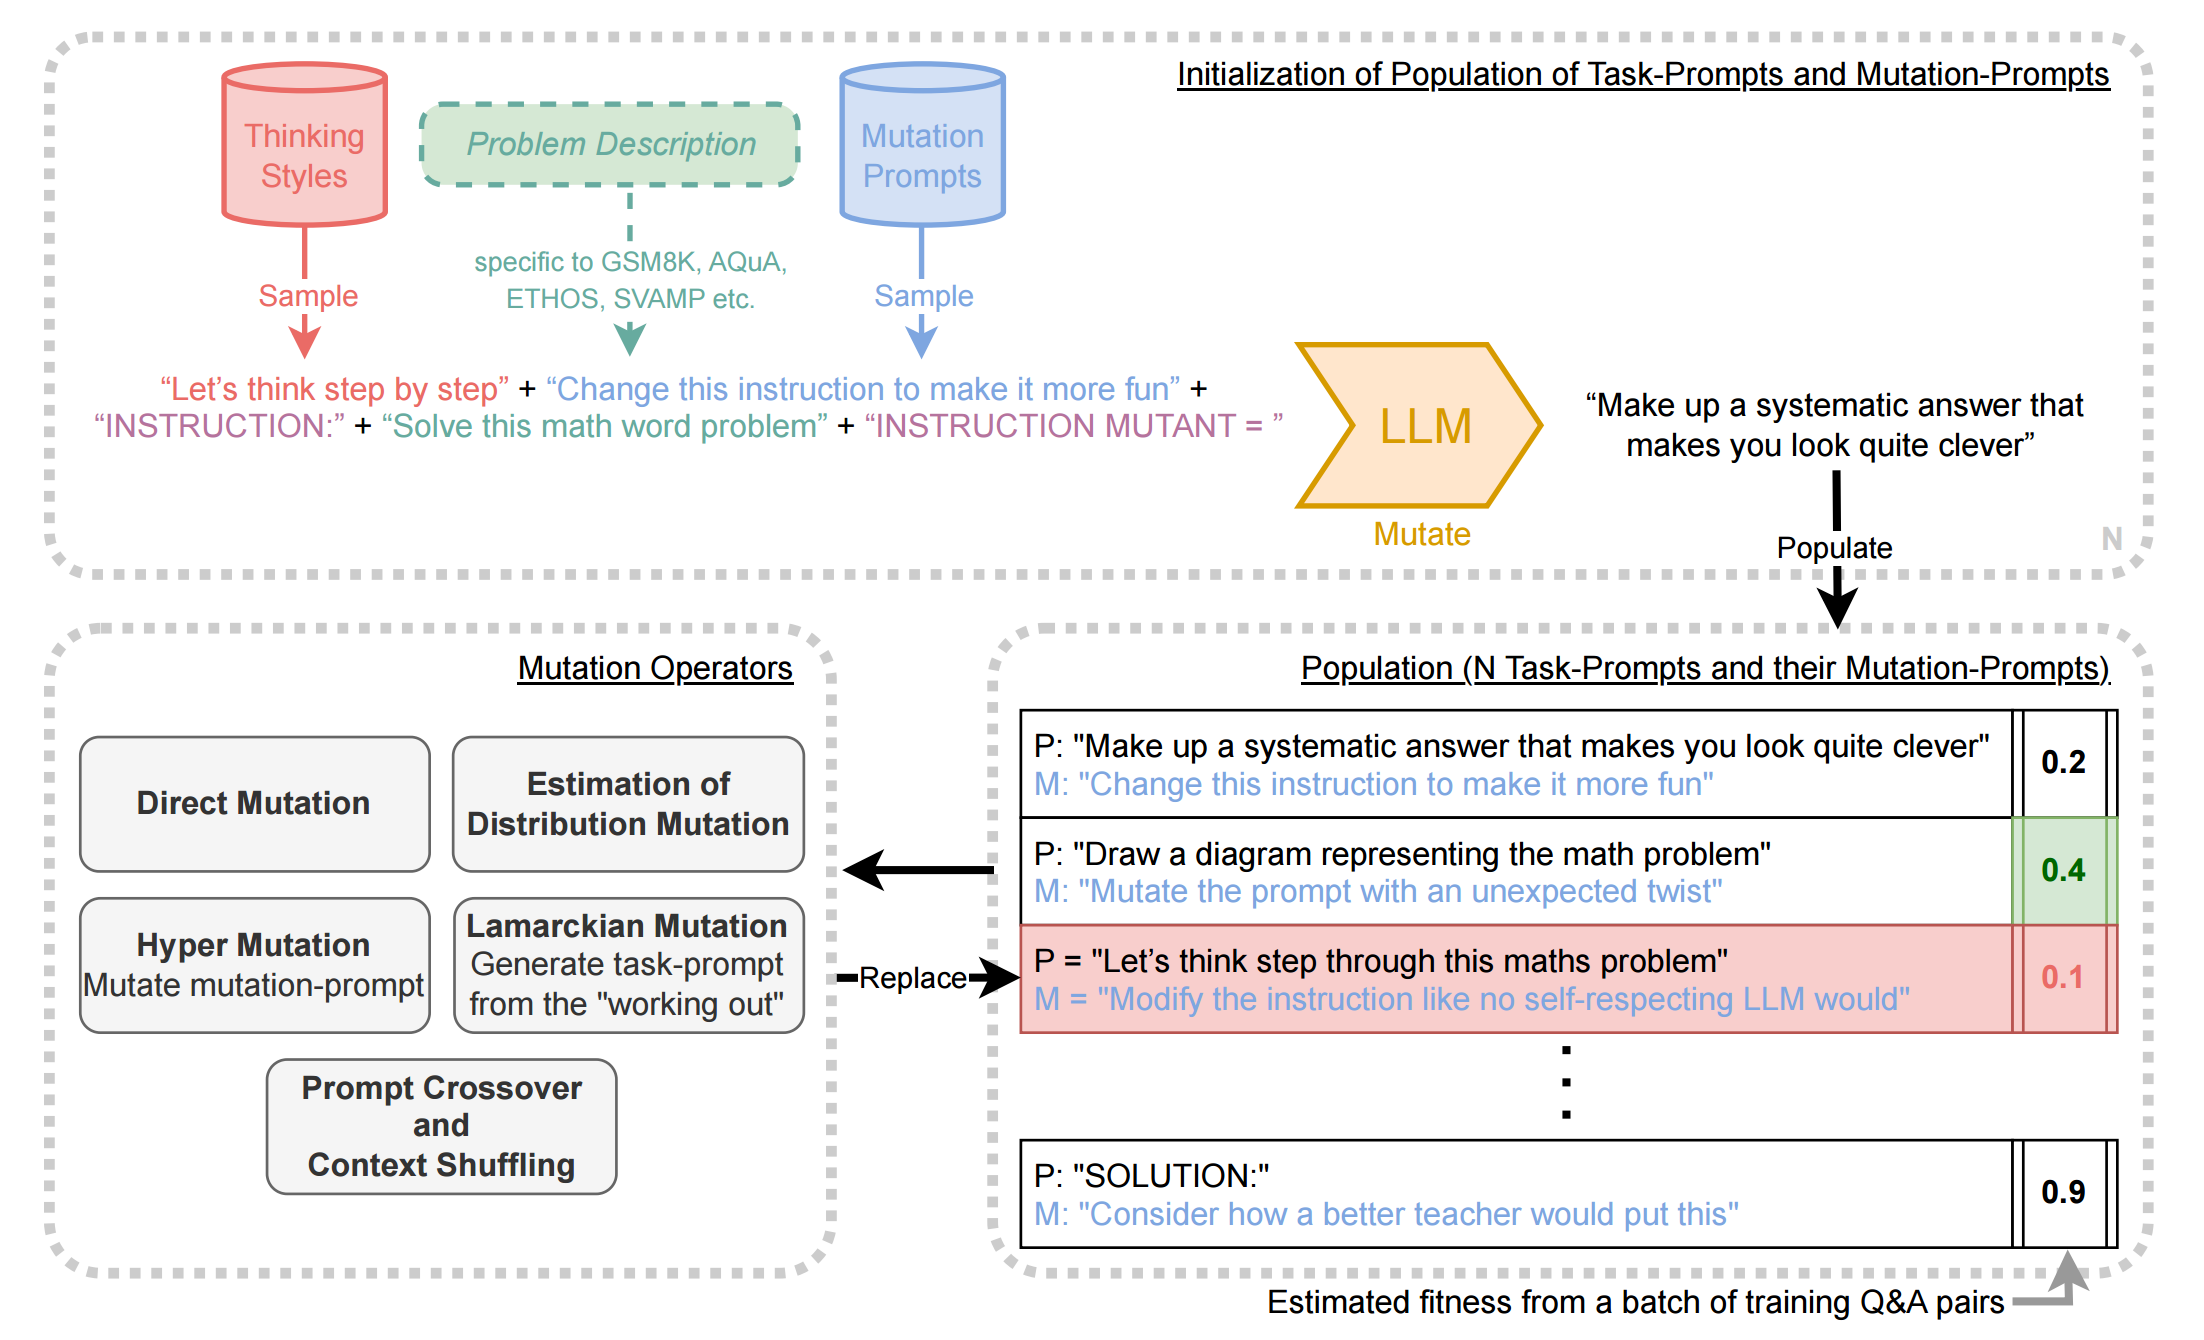
\includegraphics[width=140mm]{images/promptbreeder}
	\caption{دیاگرام روش مولد اعلان}
	\label{fig_promptbreeder}
\end{figure}

روش مولد اعلان در آزمایش‌های مختلف نشان داده است که می‌تواند از روش‌های متداول مهندسی اعلان مانند CoT و PS عملکرد بهتری داشته باشد. همچنین، این سیستم در حوزه‌های مختلف مانند حل مسائل ریاضی، استدلال عمومی
\LTRfootnote{commonsense reasoning}
، و کلاس‌بندی گفتار نفرت‌آمیز
\LTRfootnote{hate speech classification}
 بهبود چشمگیری ایجاد کرده است. مهم‌ترین مزیت آن این است که به به‌روزرسانی پارامترهای مدل نیازی ندارد و تنها از طریق اصلاح اعلان‌ها، کارایی مدل را افزایش می‌دهد.  

این روش نشان‌دهنده‌ی قدرت بهینه‌سازی خودکار اعلان‌ها و حرکت به‌سوی سیستم‌های هوش مصنوعی خودبهبوددهنده و خودارجاعی است که می‌توانند با حداقل مداخله انسانی، عملکرد خود را در طی زمان بهبود بخشند.


\section{جمع‌بندی مباحث ارائه‌شده}
این فصل با هدف بررسی پیشینه تحقیق و تبیین مفاهیم بنیادی مرتبط با موضوع پژوهش تدوین گردید. در این فصل، تلاش شد تا ضمن ارائه چارچوب نظری جامع، زمینه مناسبی برای درک بهتر مسأله تحقیق و مسیر پژوهش فراهم شود. با توجه به گستره و عمق موضوعات مطرح‌شده، می‌توان این فصل را به‌عنوان شالوده‌ای برای تحلیل‌ها و مطالعات تخصصی‌تر در فصول بعدی قلمداد نمود.

در این فصل، نخست به معرفی و تحلیل مدل‌های زبان بزرگ پرداخته شد و روند تکاملی این مدل‌ها از آغاز تا وضعیت کنونی آن‌ها مورد بررسی قرار گرفت. در ادامه، به معماری‌های رایج و کاربردهای متنوع این مدل‌ها اشاره شد و اهمیت آن‌ها در پیشبرد حوزه‌های مختلف پردازش زبان طبیعی و سامانه‌های مبتنی بر هوش مصنوعی تبیین گردید.

سپس، به موضوع مهندسی اعلان و نقش آن در بهره‌برداری مؤثر از مدل‌های زبان بزرگ پرداخته شد. در این بخش، ابتدا روش‌های سنتی مهندسی اعلان، شامل استفاده از یادگیری درون متنی، روش زنجیره تفکر ، استدلال بدون نمونه آموزشی، برنامه تفکر، بهینه سازی با اعلان و روش برنامه\/ریزی و حل به تفصیل بررسی شدند. در ادامه، به معرفی و تحلیل رویکردهای نوین در بهینه‌سازی خودکار اعلان‌ها پرداخته شد. از جمله این روش‌ها می‌توان به زنجیره تفکر خودکار، مهندسی اعلان خودکار و روش مولد اعلان اشاره نمود که هریک با هدف افزایش دقت و توان استدلال مدل‌های زبانی توسعه یافته‌اند.


بر مبنای مباحث ارائه‌شده، آشکار شد که مهندسی اعلان و بهینه‌سازی آن از مهم‌ترین مؤلفه‌ها در افزایش کارایی مدل‌های زبان بزرگ به شمار می‌رود. این امر اهمیت طراحی الگوریتم‌های نوین و کارآمد برای بهبود ساختار و محتوای اعلان‌ها را دوچندان می‌سازد.

در فصل آتی، به تشریح کامل الگوریتم پیشنهادی پرداخته خواهد شد. این الگوریتم که مولد اعلان ساده نام دارد، یکی از رویکردهای نوین در زمینه بهینه‌سازی و تکامل خودکار اعلان‌ها محسوب می‌شود و مبتنی بر اصول الگوریتم‌های تکاملی و بهبود مستمر اعلان‌ها از طریق تولید، ارزیابی و گزینش نسل‌های مختلف اعلان‌ها طراحی شده است. در فصل آینده، به‌طور دقیق به ساختار، مراحل اجرایی و مزایای این الگوریتم در مقایسه با سایر روش‌ها پرداخته خواهد شد.
